% !TEX TS-program = pdflatex
% !TEX encoding = UTF-8 Unicode

% This is a simple template for a LaTeX document using the "article" class.
% See "book", "report", "letter" for other types of document.

\documentclass[10pt]{article} % use larger type; default would be 10pt

\usepackage[utf8]{inputenc} % set input encoding (not needed with XeLaTeX)

%%% Examples of Article customizations
% These packages are optional, depending whether you want the features they provide.
% See the LaTeX Companion or other references for full information.

%%% PAGE DIMENSIONS
\usepackage{geometry} % to change the page dimensions
\geometry{a4paper} % or letterpaper (US) or a5paper or....
% \geometry{margin=2in} % for example, change the margins to 2 inches all round
% \geometry{landscape} % set up the page for landscape
%   read geometry.pdf for detailed page layout information

\usepackage{graphicx} % support the \includegraphics command and options

% \usepackage[parfill]{parskip} % Activate to begin paragraphs with an empty line rather than an indent

%%% PACKAGES
\usepackage{booktabs} % for much better looking tables
\usepackage{array} % for better arrays (eg matrices) in maths
\usepackage{paralist} % very flexible & customisable lists (eg. enumerate/itemize, etc.)
\usepackage{verbatim} % adds environment for commenting out blocks of text & for better verbatim
\usepackage{subfig} % make it possible to include more than one captioned figure/table in a single float
% These packages are all incorporated in the memoir class to one degree or another...

%%% HEADERS & FOOTERS
\usepackage{fancyhdr} % This should be set AFTER setting up the page geometry
\pagestyle{fancy} % options: empty , plain , fancy
\renewcommand{\headrulewidth}{0pt} % customise the layout...
\lhead{}\chead{}\rhead{}
\lfoot{}\cfoot{\thepage}\rfoot{}

%%% SECTION TITLE APPEARANCE
\usepackage{sectsty}
\allsectionsfont{\sffamily\mdseries\upshape} % (See the fntguide.pdf for font help)
% (This matches ConTeXt defaults)

%%% ToC (table of contents) APPEARANCE
\usepackage[nottoc,notlof,notlot]{tocbibind} % Put the bibliography in the ToC
\usepackage[titles,subfigure]{tocloft} % Alter the style of the Table of Contents
\renewcommand{\cftsecfont}{\rmfamily\mdseries\upshape}
\renewcommand{\cftsecpagefont}{\rmfamily\mdseries\upshape} % No bold!

 \usepackage{multirow}

%%% END Article customizations

\usepackage{listings}
\usepackage{float}
\usepackage{parskip}% http://ctan.org/pkg/parskip
\usepackage{amsmath}
\usepackage{amsfonts}
\usepackage{amssymb}

%%% The "real" document content comes below...

\title{PRISMS-PF User Guide (v2.0)}
\author{Stephen DeWitt (prismsphasefield.dev@umich.edu)}
%\date{} % Activate to display a given date or no date (if empty),
         % otherwise the current date is printed 

\begin{document}
\maketitle

\tableofcontents

\clearpage

\section{Overview}
PRISMS-PF is an open-source finite element simulation code with a focus on solving equations from phase field models. It is being developed as part of the PRISMS Center at the University of Michigan. PRISMS-PF is built on top of the popular and powerful deal.II finite element library. PRISMS-PF was developed to make high performance phase field simulation capabilities available to the wider scientific community with an easy-to-use and easy-to-learn interface. Benchmark tests show that even without its adaptive meshing capabilities PRISMS-PF is competitive with specialized finite difference codes written in Fortran with MPI parallelization in terms performance,  and in some cases runs several times faster. PRISMS-PF can be used to solve a wide variety of systems of coupled parabolic partial differential equations (e.g. the diffusion equation) and elliptic partial differential equations (e.g. Poisson's equation). With PRISMS-PF, you have access to adaptive meshing and parallelization that has been demonstrated on over a thousand processors. Moreover, the matrix-free framework from deal.II allows much larger than typical finite element programs -- PRISMS-PF has been used for calculations with over one \emph{billion} degrees of freedom.

This user guide starts with instructions for downloading PRISMS-PF and install the necessary prerequisites. Next are instructions for running the built-in example applications and visualizing the results. A detailed look at the input files follows, and the guide finishes with some instructions on how to create your own PRISMS-PF applications.

If you run into any issues not covered by this guide, or have any questions, please send an email to the PRISMS-PF email list: prisms-pf-users@googlegroups.com. If you'd like to contact the PRISMS-PF developers directly, send an email to: prismsphaseField.dev@umich.edu.

PRISMS-PF was developed as part of the PRedictive Integrated Structural Materials Science (PRISMS) Center at University of Michigan which is supported by the U.S. Department of Energy (DOE), Office of Basic Energy Sciences, Division of Materials Sciences and Engineering under Award \#DE-SC0008637.

\section{Downloading deal.II and PRISMS-PF}

Before downloading PRISMS-PF itself, one should install CMake and deal.II. CMake can be downloaded at: https://cmake.org/download, which also has installation instructions. Be sure to add CMake to your path by entering:
\begin{lstlisting}
$ $ PATH="/path/to/cmake/Contents/bin":"$PATH"
\end{lstlisting}
filling in the path to the installation of CMake (for example, on Mac OS, the default installation path is /Applications/CMake.app/Contents/bin). For convience, we recommend adding this line to your bash profile. Your bash profile can be opened via the following terminal command
\begin{lstlisting}
$ vi ~/.profile
\end{lstlisting}

Deal.II can be downloaded at https://www.dealii.org/download.html, which also has instructions. The deal.II installation process depends on your operating system. PRISMS-PF has been tested with Deal.II versions 8.3.0 through 8.5.0. We recommend using deal.II 8.4.2, if possible. If you use deal.II 8.5.0, expect to recieve a number of warnings during compilation (discussed in Sec. \ref{running_examples}) about functions used in PRISMS-PF that are deprecated in deal.II 8.5.0.

\subsection{Installing deal.II for Mac OS X}
A binary package for version 8.4.2 (and other versions) is available at https://github.com/dealii/dealii/releases. The binary package includes all the libraries that you need (excluding CMake). To install deal.II open the .dmg file and drag ``deal.II.app'' into your Applications folder. Then, open ``deal.II.app'', which will open a Terminal window and set the necessary environment variables. You may need to modify your security settings so that your operating system will let you open the application (in System Preferences, select Security $\&$ Privacy, then under the general tab choose to allow apps downloaded from anywhere; don't click ``Open deal.II.app anyway'', we have found that doing so doesn't actually launch deal.II.app). 

In some cases, deal.II.app will not open, possibly freezing at the ``Verifying...'' stage. If this happens, right click on it and select ``Show Package Contents''. Then go to ``/Contents/Resources/bin/'' and launch ``dealii-terminal''. This should launch the Terminal window that sets the environment variables.

We have found that for some older versions of Mac OS are incompatible with deal.II version 8.4.2 (due to the version of the Clang compiler that is installed by default). In those cases we recommend downloading this version 8.3.0 package:
\\ https://github.com/dealii/dealii/releases/download/v8.3.0/dealii-8.3.0.nocxx14.dmg.

\subsection{Installing deal.II for Linux}
Unfortunately, on a Linux machine you will likely have to compile and install deal.II from the source. The source code for version 8.4.2 can be downloaded at https://github.com/dealii/dealii/releases. Detailed installation directions can be found at https://www.dealii.org/8.5.0/readme.html. For some versions of Linux, packages are available (Gentoo, Debian testing (stretch), and Ubuntu 16.10+). See https://www.dealii.org/download.html for details.

Below we list instructions for installing deal.II and its prerequisites both manually and using candi, an automatic deal.II installation script. For now, we recomend the traditional route, because we haven't been able to get candi to consistently work. Recently, deal.II has been made available on Linuxbrew. We have not tried this yet, but it may be a good option. Details can be found at https://github.com/dealii/dealii/wiki/deal.II-on-Homebrew---Linuxbrew.

\subsubsection{Traditional Installation (Recommended assuming no package is available)}
Before building deal.II, you will need to install two libraries, MPI and p4est. Make sure you have both libraries installed before installing deal.II, or else you will have to reinstall deal.II! Many computing clusters already have these libraries installed. MPI libraries (such as MPICH2) are often available through package managers (e.g. yum, apt, pkg$\_$add, port, brew), installing it using your package manager of choice is likely the simplest option. If not, you can find binaries and the source code at http://www.mpich.org/downloads/, as well as instructions for installation. The p4est library may also be available through your package manager. If not, you can download the latest release tarball at http://www.p4est.org/. To install, unzip the archive, move to the p4est root directory and enter the following commands at the command line:
\begin{lstlisting}
$ ./configure --enable-mpi; make; make install
\end{lstlisting}
Users have found that this approach works better than the setup script ``p4est-setup.sh'' that is on the deal.ii website. More detailed installation instructions can be found in the ``INSTALL'' and ``README'' files in the p4est root directory.

With MPI and p4est installed, you are ready to install deal.II. Open the archive you downloaded from the deal.II website. From the root deal.II directory enter the following commands:
\begin{lstlisting}
$ mkdir build
$ cd build
$ cmake -DP4EST_DIR=/path/to/installation/dir -DDEAL_II_WITH_P4EST=ON 
-DDEAL_II_WITH_MPI=ON -DCMAKE_INSTALL_PREFIX=/path/to/install/dir
$ make install
\end{lstlisting}
where ``/path/to/install/dir'' is the path to where you want to install deal.II. After installation is complete (which can take take up to an hour), open the file ``summary.log''. The second section of the log file lists the configured features. Ensure that DEAL$\_$II$\_$WITH$\_$MPI and DEAL$\_$II$\_$WITH$\_$P4EST say either ``set up with bundled packages'' or ``set up with external dependences''. If either is listed as ``OFF'', then deal.II was unable to find MPI or p4est. If this is the case, double check that MPI and p4est were installed correctly. 

\subsubsection{Using candi}
An alternative route is to use the following candi (compile and install) script to install deal.II and its prerequisites: \\
https://github.com/koecher/candi \\

If it works, it should be much simpler than the traditional route described above. However in limited attempts, we have not been able to successfully install deal.II with candi. After more testing and/or consultation with the developer, we hope to make this a plausible option.

\subsection{Downloading PRISMS-PF}
PRISMS-PF is available for download at our GitHub site: https://github.com/prisms-center/phaseField. The recommended method for downloading the PRISMS-PF source code is through git. Using a Linux/Unix terminal, go to the directory where you want PRISMS-PF to be located. To clone the repository, type:
\begin{lstlisting}
$ git clone https://github.com/prisms-center/phaseField.git
\end{lstlisting}
Git will then download the PRISMS-PF source code into a directory entitled ``phaseField''. A resource for learning to use Git can be found at: \\https://git-scm.com/book.

If you prefer not to use Git, a zip file containing the PRISMS-PF source code can be downloaded at: \\https://github.com/prisms-center/phaseField/releases.

\section{Running the Example Applications} \label{running_examples}
\subsection{The Example Applications}
After deal.II and PRISMS-PF are downloaded, you can run the pre-built PRISMS-PF example applications. At this time, the example applications include:
\begin{itemize}
\item allenCahn: An implementation of the Allen-Cahn equation for two phases. (2D)
\item allenCahn\_pfield: Like allenCahn, but loads in initial conditions using PRISMS IntegrationTools. (2D)
\item cahnHilliard: An implementation of the Cahn-Hilliard equation for two phases. (2D)
\item cahnHilliardWithAdaptivity: Like cahnHilliard, but with adaptive meshing enabled. (2D)
\item coupledCahnHilliardAllenCahn: An implementation of the coupled Cahn-Hilliard/Allen-Cahn set of equations. (2D)
\item CHAC\_anisotropy: Coupled Cahn-Hilliard/Allen-Cahn equations with weakly anisotropic interfacial energy. (2D)
\item CHAC\_anisotropyRegularized: Like CHAC\_anisotropy, but with a regularization term to permit strongly anisotropic interfacial energy. (2D)
\item fickianDiffusion: An implementation of the diffusion equation with a time-dependent source term. (2D)
\item mechanics: An implementation of linear elasticity for a material in uniaxial tension. (3D)
\item CHiMaD\_benchmark1a: An implementation of the CHiMaD spinodal decomposition benchmark problem. (2D)
\item CHiMaD\_benchmark2a: An implementation of the CHiMaD Ostwald ripening benchmark problem. (2D)
\item CHiMaD\_benchmark6a: An implementation of the CHiMaD electrochemistry benchmark problem. (2D)
\item CHiMaD\_benchmark6b: An implementation of the CHiMaD electrochemistry benchmark problem with a curved domain. (2D)
\item dendriticSolidification: An implementation of a solidification model for a pure material resulting in the growth of a dendrite. (2D)
\item eshelbyInclusion: An implementation of linear elasticity for a spherical inclusion. (3D)
\item grainGrowth: An implementation of ten coupled Allen-Cahn equations simulating grain growth in two dimensions. (2D)
\item precipiateEvolution: An implementation of the coupled Cahn-Hilliard/Allen-Cahn/Linear Elasticity equations often used in phase field simulation of precipitate evolution. (2D)
\item precipiateEvolution\_pfunction: Like precipitateEvolution, but loads inputs using PRISMS IntegrationTools. (2D)
\item singlePrecipitateKKS: Similar to precipiateEvolution, but uses the KKS model rather than the WBM model for the free energy functional. (3D)
\item nucleationModel: KKS precipitation model that makes use of the PRISMS-PF explicit nucleation capabilities. (2D)
\item preferential\_nucleationModel: Like nucleationModel, but with a zone with an increased nucleation rate to simulate a grain boundary. (2D)
\end{itemize}

A directory for each of these applications can be found in the applications directory (i.e. phaseField/applications). The applications contain a formulation file giving the governing equations. In addition to the 21 applications listed above, some application names may be preceded by an underscore. The underscore is used to denote applications that are still under active development.

\subsection{Compiling the Core PRISMS-PF Library}
After downloading PRISMS-PF, we recommend that you compile the core library (see note at the end of this section). To do so, enter the root PRISMS-PF directory from the directory where you downloaded it to, run CMake, and then compile the library:
\begin{lstlisting}
$ cd phaseField 
$ cmake .
$ make -j 8 
\end{lstlisting}
In the last command, the number following ``-j'' is the number of threads used during compilation. The general rule of thumb is to pick a number 1.5$\times$ the number of processors available. This process should take a minute or two and will compile both the ``debug'' and ``release'' versions of the core PRISMS-PF library (see \ref{release_multicore}).

Note: This step can be skipped and the core library will be compiled the first time that you compile one of the applications. However, the compilation will be on a single thread and thus will take much longer than if you follow the instructions above and use multiple threads.

\subsection{Running the Allen-Cahn Example Application} \label{allen_cahn_instructions}
From the ``phaseField'' directory one can run the Allen-Cahn example application through to following terminal commands:
\begin{lstlisting}
$ cd applications/allenCahn/ 
$ cmake . 
$ make debug 
$ mpirun -n 1 main 
\end{lstlisting}

The first command moves from the ``phaseField'' directory to the directory of the Allen-Cahn example. The second command checks that core PRISMS-PF library has been compiled, (re-)compiles it if necessary, and creates a \emph{makefile} using CMake. The third command compiles the executable in ``debug'' mode, which enables a number of exception checks in the code and adds debugging information that can be used by a debugger (e.g. gdb). The fourth command runs the program using a single processor.

As the program runs, information from each time step outputs to the terminal window. After the simulation is complete, a summary the time taken in a few major sections of the code and the total wall time is printed to the terminal window. 

Here is a screenshot of typical output from CMake as you create the \emph{makefile}:
\begin{figure}[H]
\vspace{-70pt}
%\centering
\hspace{-2cm}
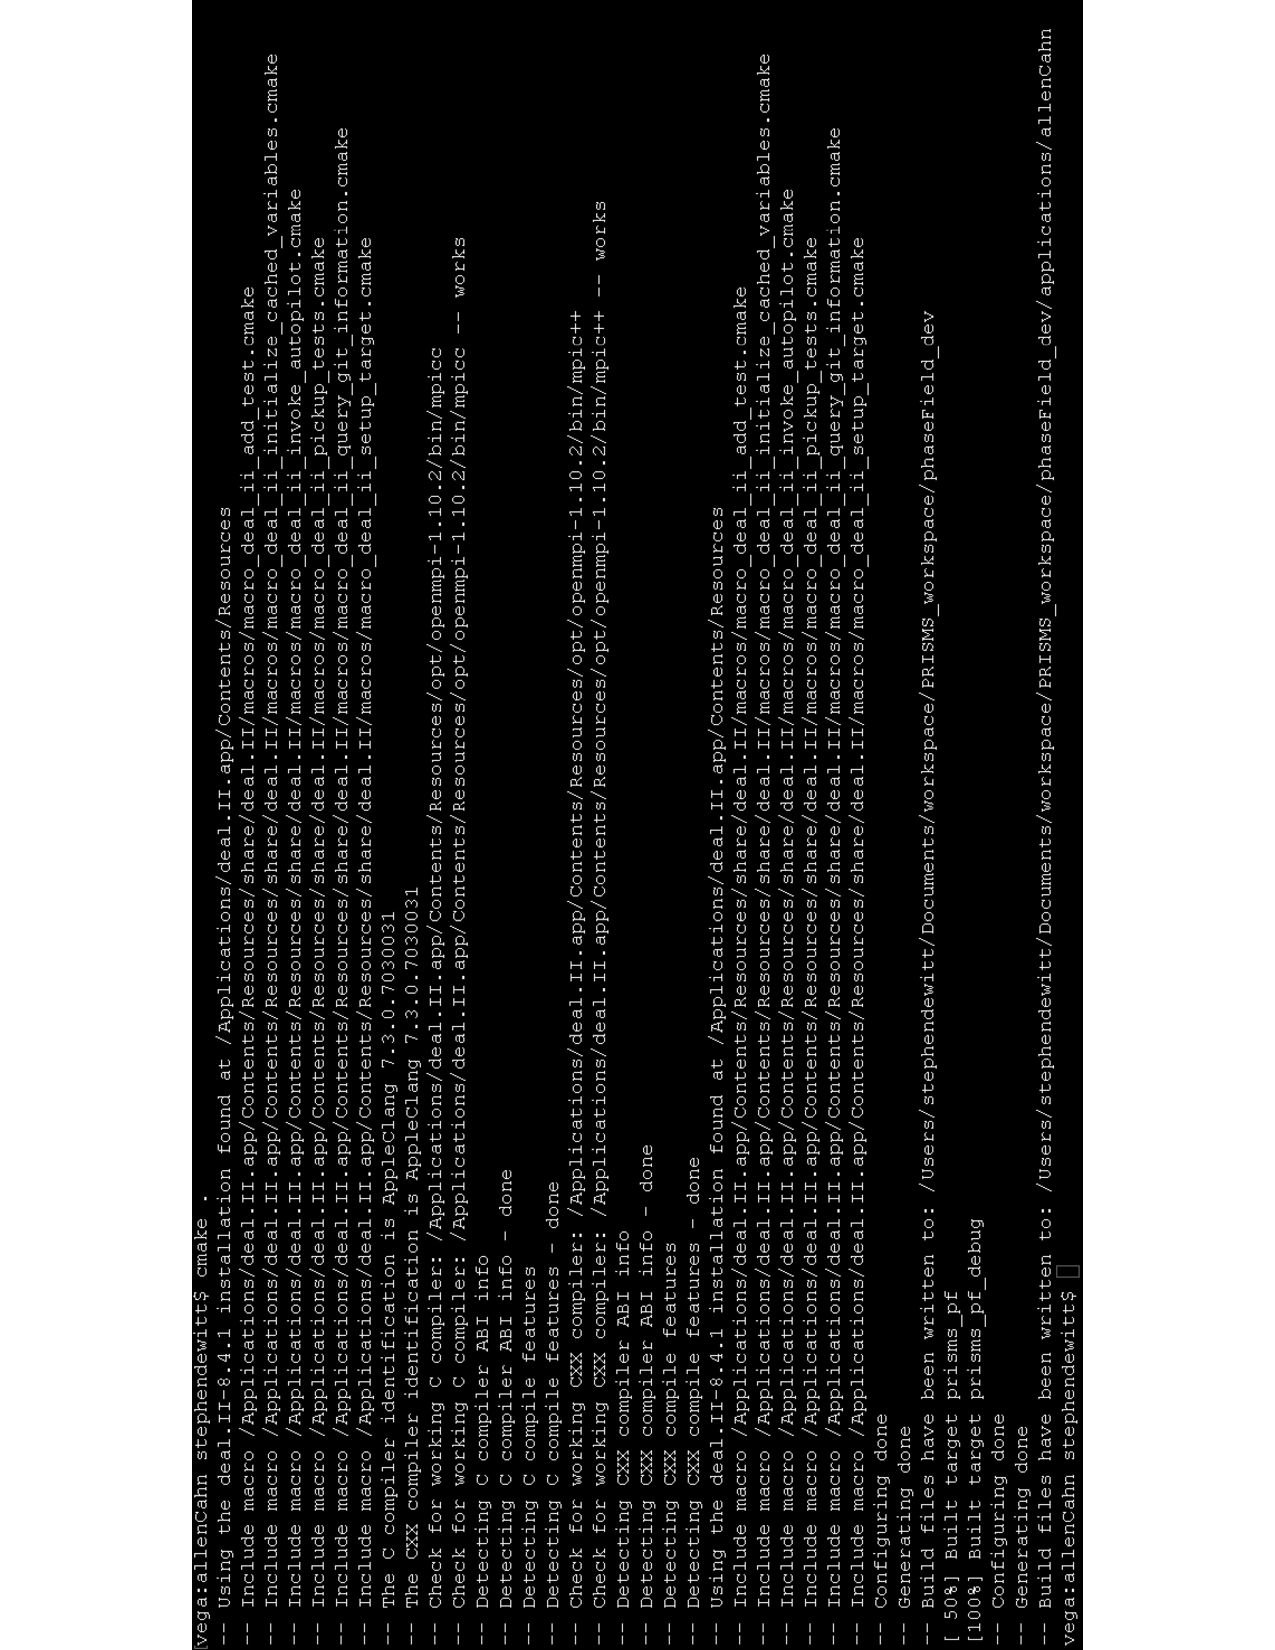
\includegraphics[height=1.3\textwidth,trim={0 0 0cm 0cm},clip,angle=-90]{cmake_output_v2}
\vspace{-70pt}
\end{figure}
Don't worry if the output isn't exactly the same as what you see, the details of some of the messages depend on your operating system and which compilers you have installed. The important part is that the bottom three messages are ``Configuring done'', ``Generating done'', and ``Build files have been written to: ...''. In the future, entering ``\$ cmake .'' will result in a shorter set of messages because CMake caches some variables from the last time it was run. As a result, you can omit the CMake step for future simulations as long as the path name to your current directory is unchanged and your installation of deal.II is unchanged.

Here is a screenshot of typical output from the compiler as you compile the executable:
\begin{figure}[H]
\vspace{0pt}
%\centering
\hspace{-2cm}
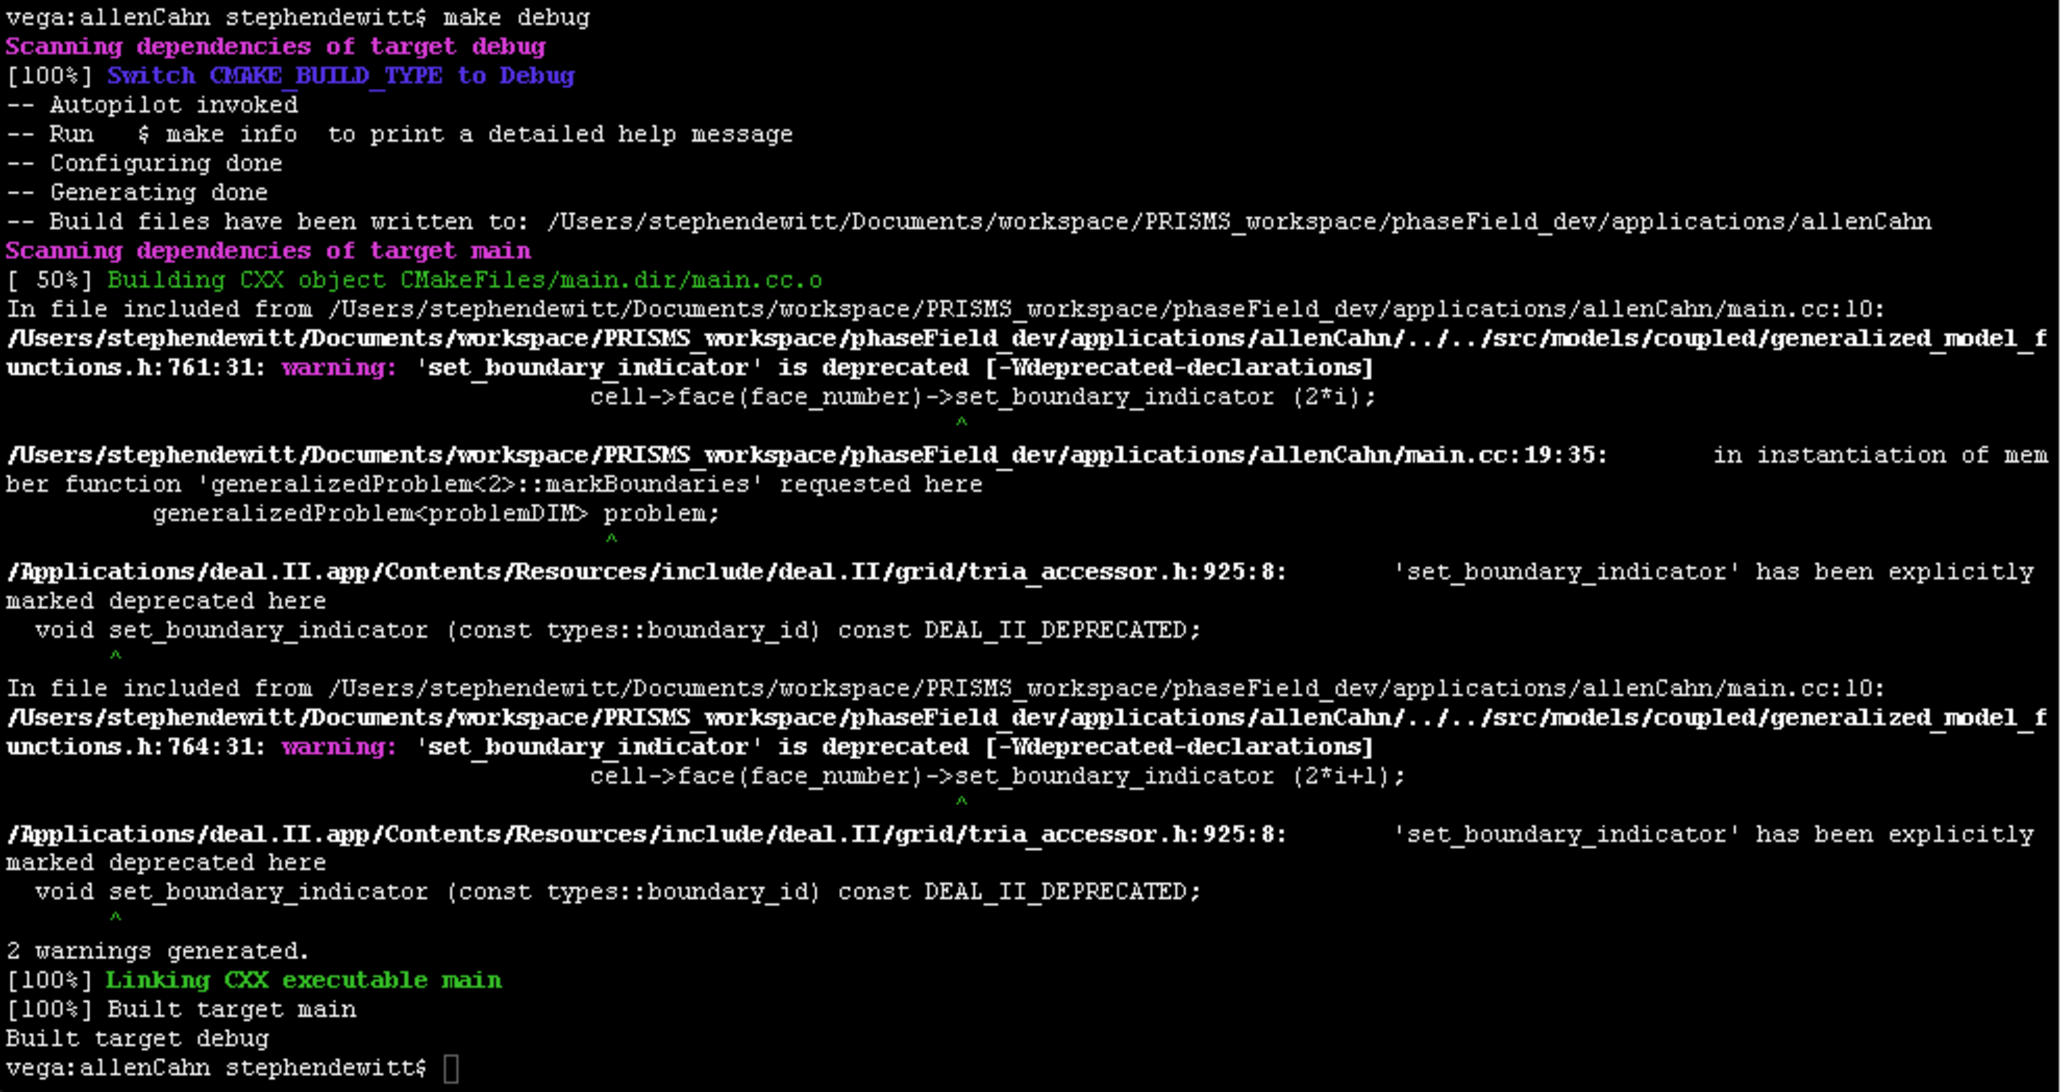
\includegraphics[width=1.3\textwidth]{compile_output}
\vspace{0pt}
\end{figure}
Depending on your version of deal.II, different warnings may appear as you compile. Common warnings include the use of functions that deal.II has marked as depricated (as in the screenshot above) and unused type definitions. In this case, PRISMS-PF uses these functions for backward compatability with deal.II version 8.4.x. We will switch to the updated functions in the near future.

Once the simultation is complete, the terminal output at the end of the simulation should look like:
\begin{figure}[H]
\vspace{-60pt}
\centering
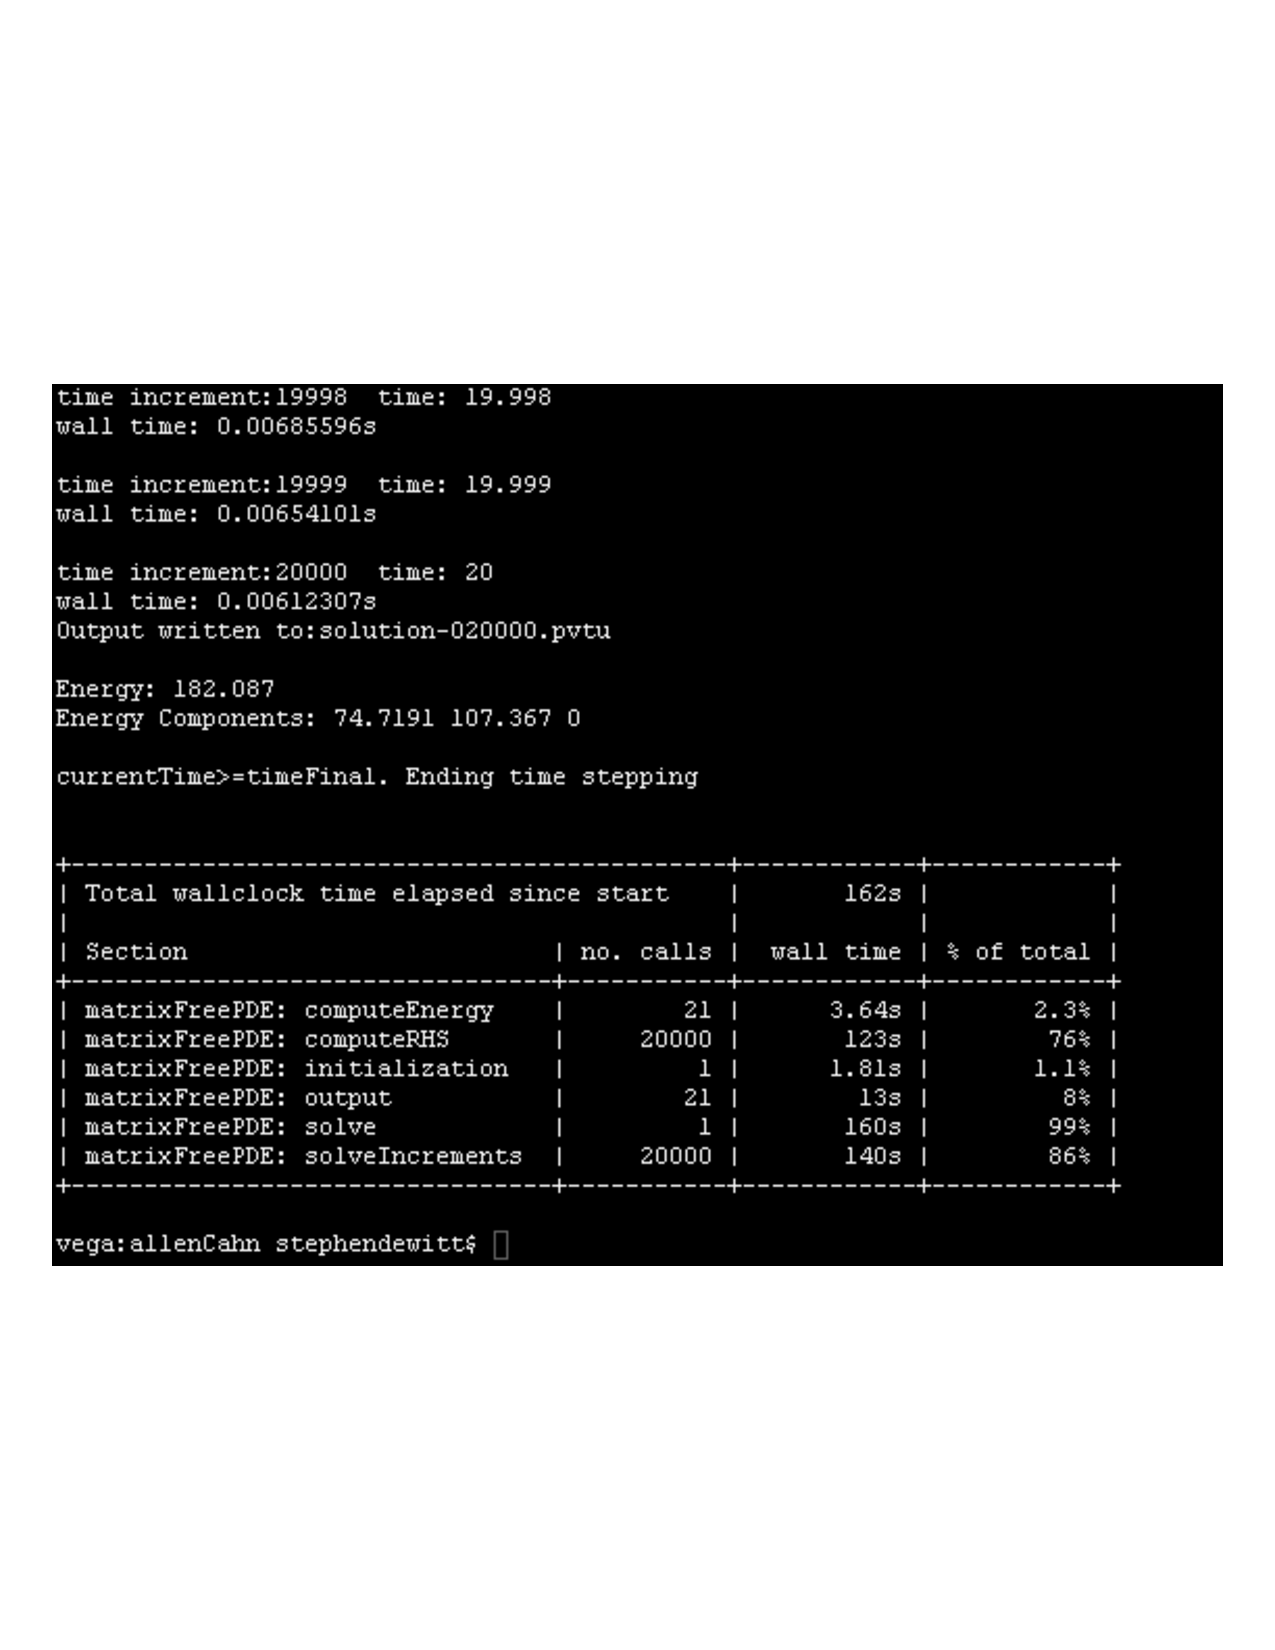
\includegraphics[width=0.9\textwidth]{allenCahn_output}
\vspace{-60pt}
\end{figure}

\subsection{What Can Go Wrong}
If you were able to enter all of the commands in the previous section and get output similar to the screenshots, congratulations! you just ran your first PRISMS-PF simulation. If not, you may be experiencing one of the common issues listed below.

If CMake gives an error message like this:
\begin{figure}[H]
\vspace{-90pt}
\centering
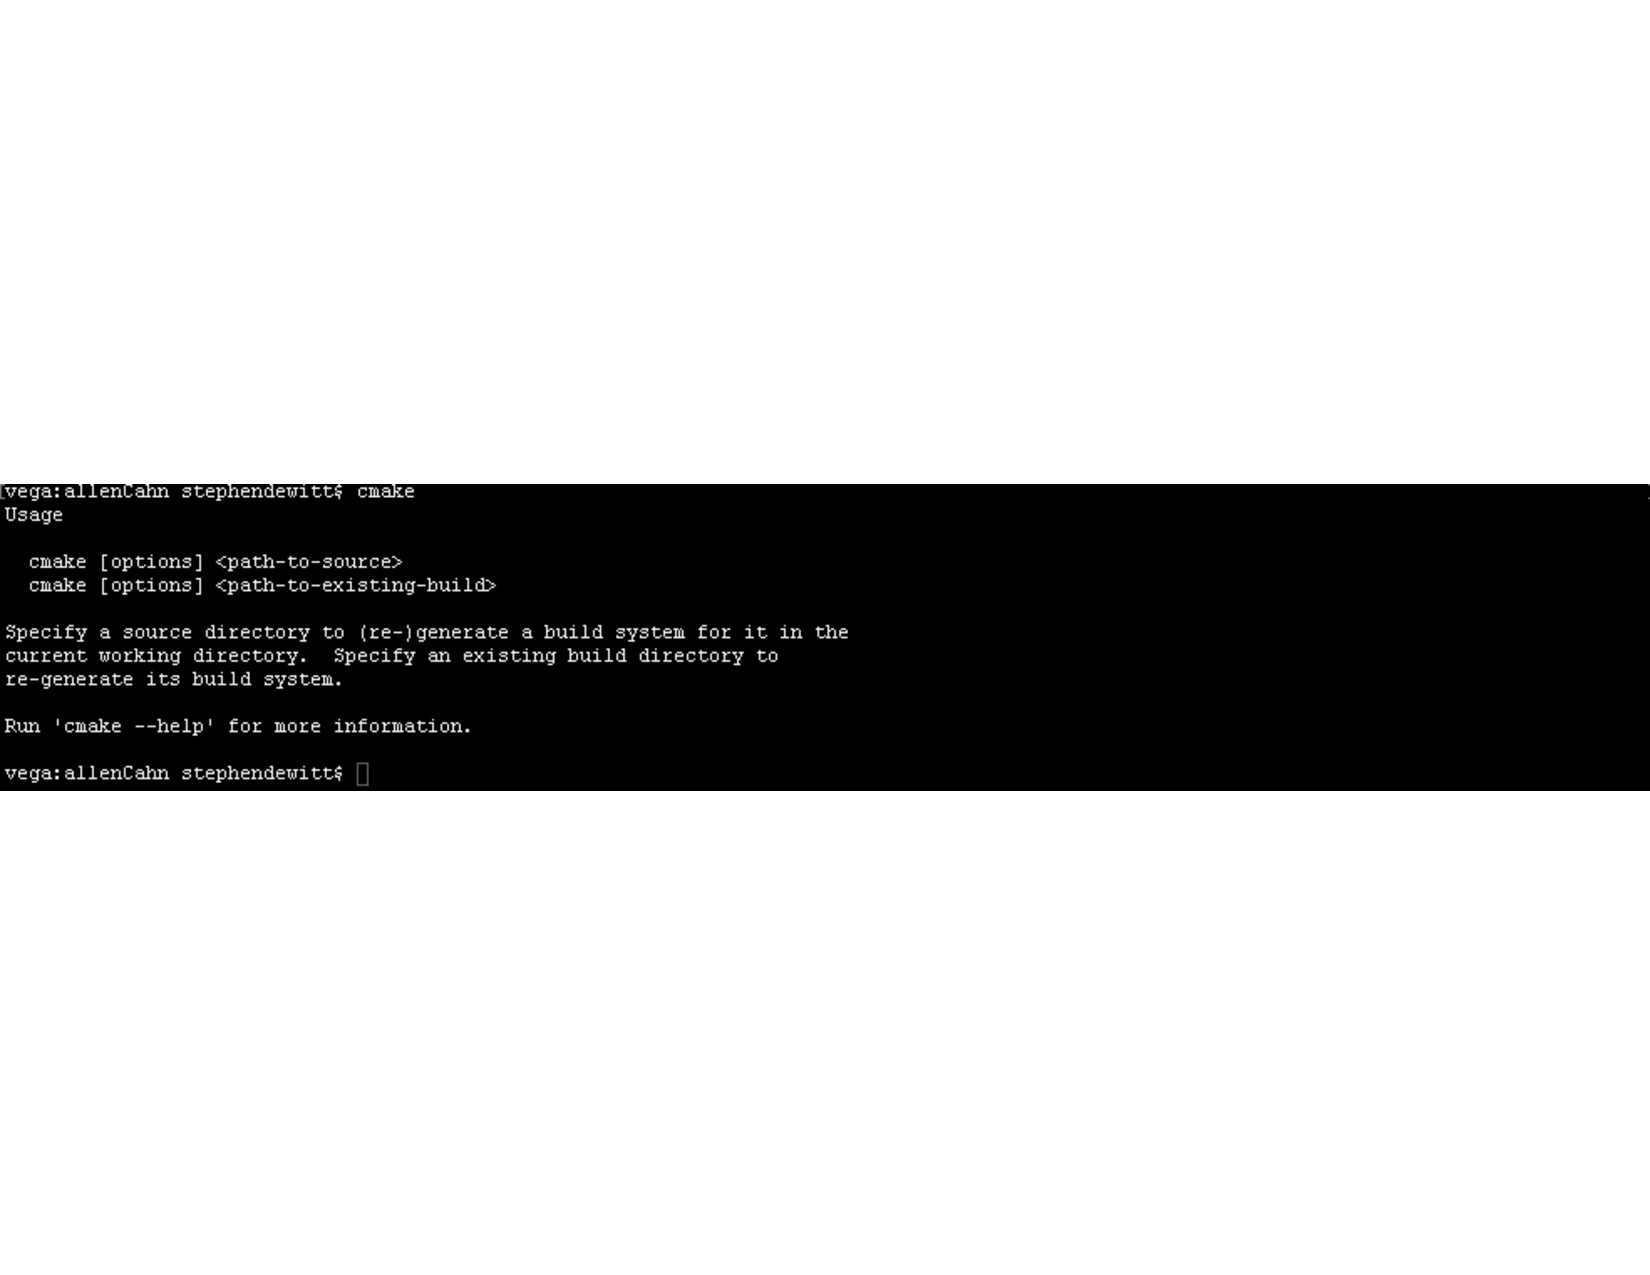
\includegraphics[width=0.9\textwidth,trim={0 0 12cm 0},clip]{cmake_no_period}
\vspace{-90pt}
\end{figure}
Then you likely forgot the period at the end of the command ``\$ cmake .''.

If CMake gives an error message like this:
\begin{figure}[H]
\vspace{-90pt}
\centering
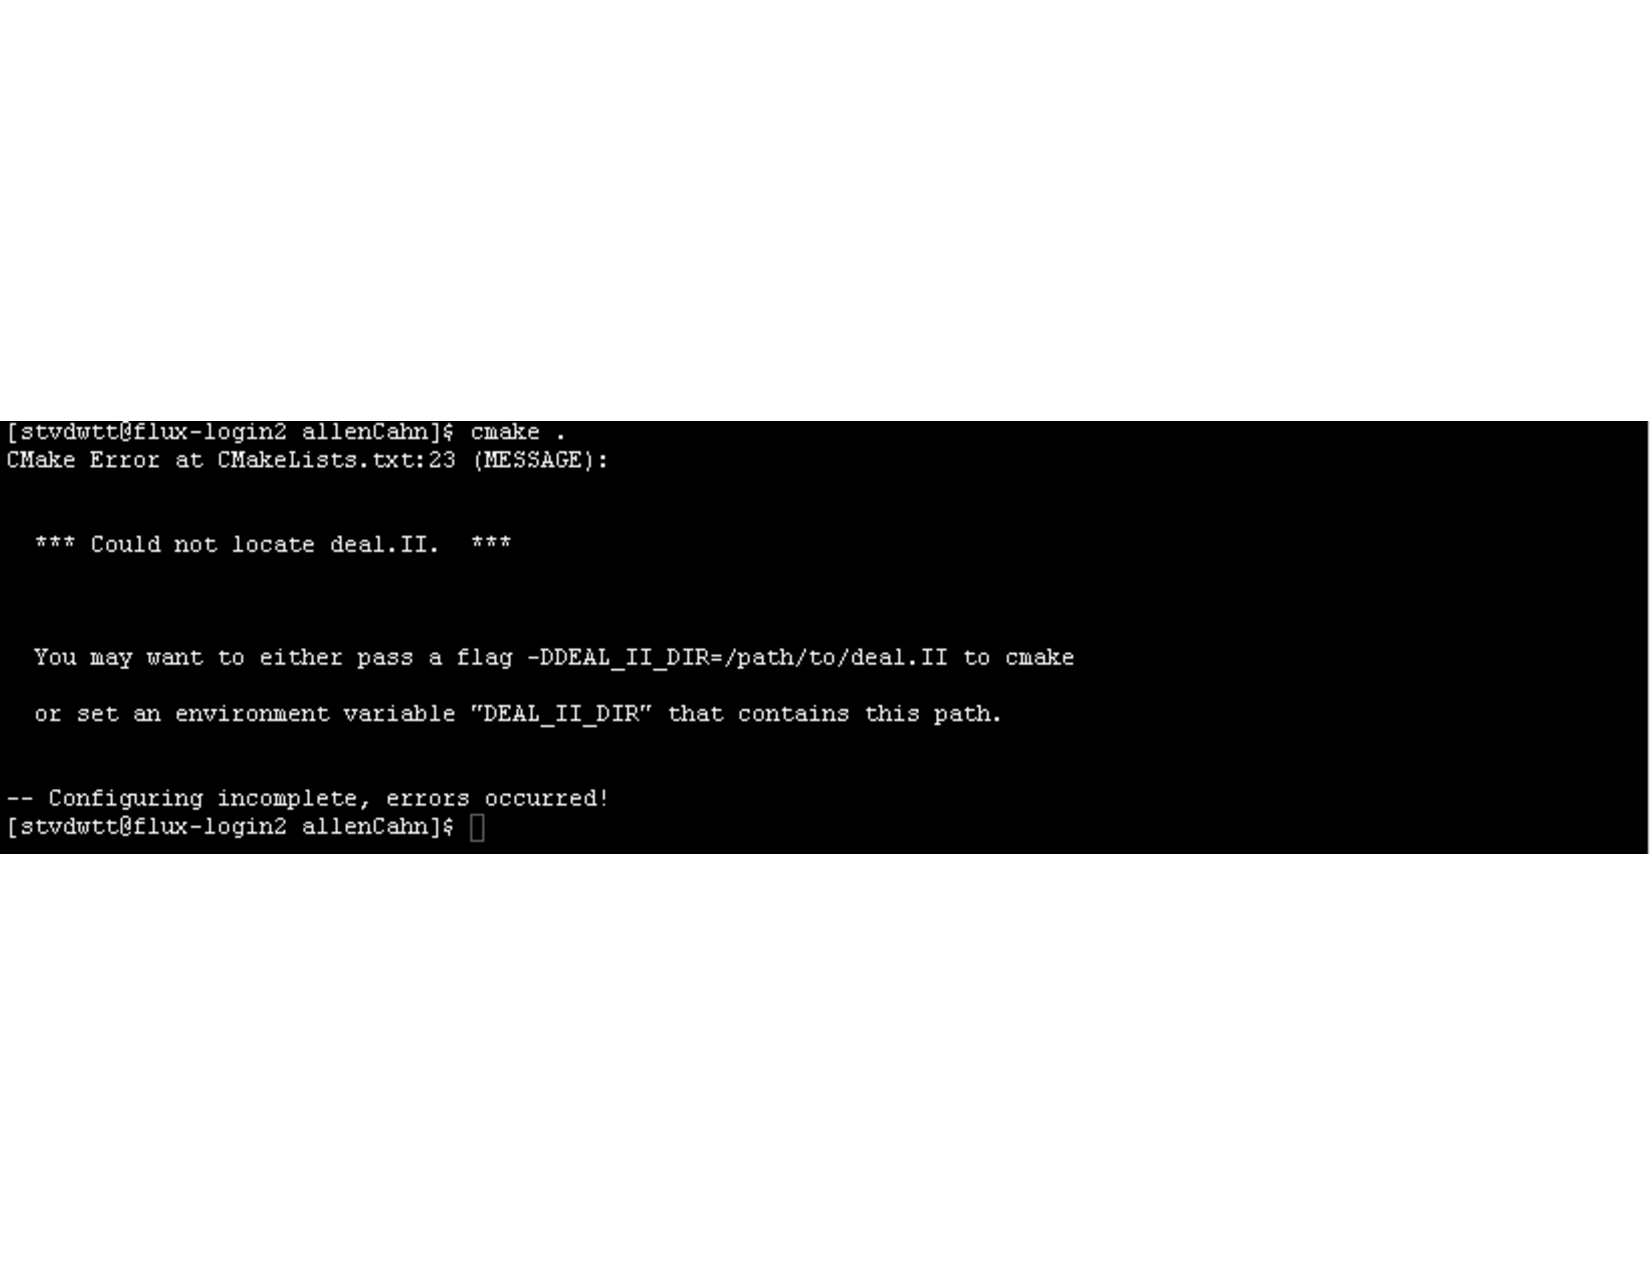
\includegraphics[width=0.9\textwidth,trim={0 0 8cm 0},clip]{cmake_no_dealii}
\vspace{-90pt}
\end{figure}
CMake cannot find your installation of deal.ii. This issue is probably caused by the lack of an environment variable pointing to the directory containing your deal.II library. You can check this with the following command:
\begin{lstlisting}
$ echo $DEAL_II_DIR
\end{lstlisting}
The terminal should then output the path to the deal.II library. For example in Mac OS, the deal.II directory may be ``/Applications/deal.II.app/Resources''. If  DEAL\_II\_DIR contains a path, go there to see if deal.II is actually installed there. If DEAL\_II\_DIR is incorrect or empty, you should set it to the directory of the correct path of your deal.II installation with the following command:
\begin{lstlisting}
$ export DEAL_II_DIR=/path/to/dealii
\end{lstlisting}
Environment variables are erased when you close your shell. To have this path set every time you open a shell (i.e. every time you open a new terminal window), you can add the command above to your shell profile (e.g. .bashrc if you use a bash shell). If you are still having problems, there may be an issue with your deal.II installation. Please consult the deal.II website for instructions.

If CMake cannot successfully detect a C++ compiler, it will generate an error message. The most common cause for this is that the machine runs the Mac OS operating system with an outdated version of the Clang compiler. Upgrading your OS to version 10.11 or newer, updating Xcode, and (re)installing the Xcode command line tools may help. Alternatively, you can install a certain version of the deal.II package that was developed to sidestep this issue:
\\https://github.com/dealii/dealii/releases/download/v8.3.0/dealii-8.3.0.nocxx14.dmg\\

Most of issues users have had are during the CMake step. If the fixes suggested above don't work for your or you have an issue not covered by this list, please contact the PRISMS-PF users list: prisms-pf-users@googlegroups.com. If you are not already on the list, please submit a join request through Google Groups or send an email with ``SUBSCRIBE'' in the subject line to prismsphasefield.dev@umich.edu. As users come across new issues, we will add them (and suggested fixes) to this section.

\subsection{Visualizing the Results of the Simulation}
Once you have successfully run a simulation, you will likely want to visualize the results.  PRISMS-PF output files are generated in the popular VTK format, as a series of *.vtu and *.pvtu files. Two common open-soure, multi-platform visualization tools for these types of files are VisIt and ParaView. Instructions for downloading this software can be found at their respective websites:
\\VisIt: https://wci.llnl.gov/simulation/computer-codes/visit/
\\ParaView: http://www.paraview.org/

To get you started, here is a brief tutorial on how to use VisIt to visualize your simulation results. For more detailed instructions, please consult the VisIt manual:
\\ https://wci.llnl.gov/simulation/computer-codes/visit/manuals

After launching the VisIt application, click ``Open'' and find the directory for the Allen Cahn example:
\begin{figure}[H]
\vspace{0pt}
\centering
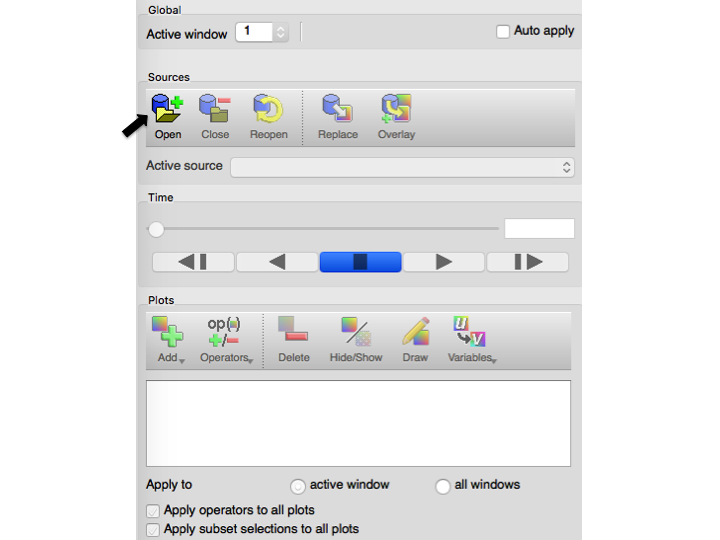
\includegraphics[width=0.7\textwidth]{visit_open.png}
\vspace{0pt}
\end{figure}
and select ``solution-*.pvtu:
\begin{figure}[H]
\vspace{0pt}
\centering
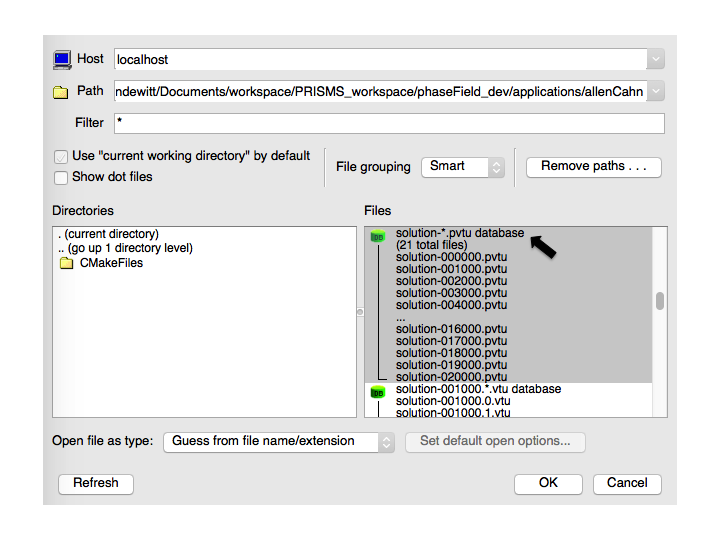
\includegraphics[width=0.7\textwidth]{visit_path.png}
\vspace{0pt}
\end{figure}
Next, click ``Add'', hover over ``Pseudocolor'', and select ``n'':
\begin{figure}[H]
\vspace{0pt}
\centering
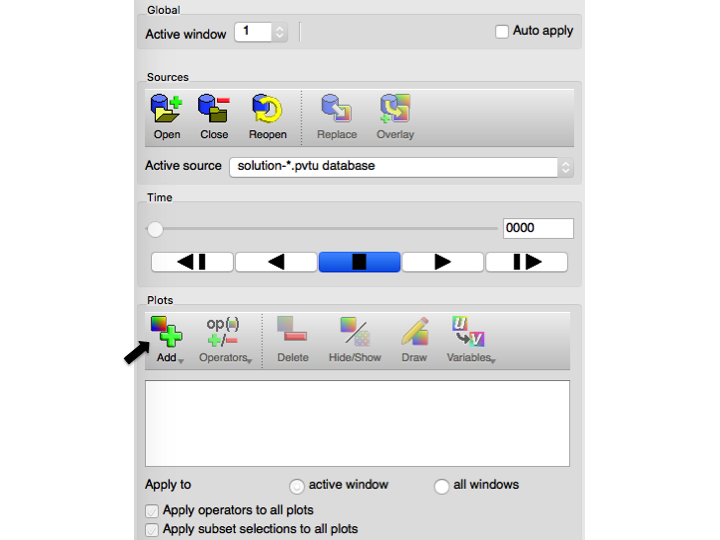
\includegraphics[width=0.7\textwidth]{visit_add.png}
\vspace{0pt}
\end{figure}
Next, click ``Draw'' to make a plot:
\begin{figure}[H]
\vspace{0pt}
\centering
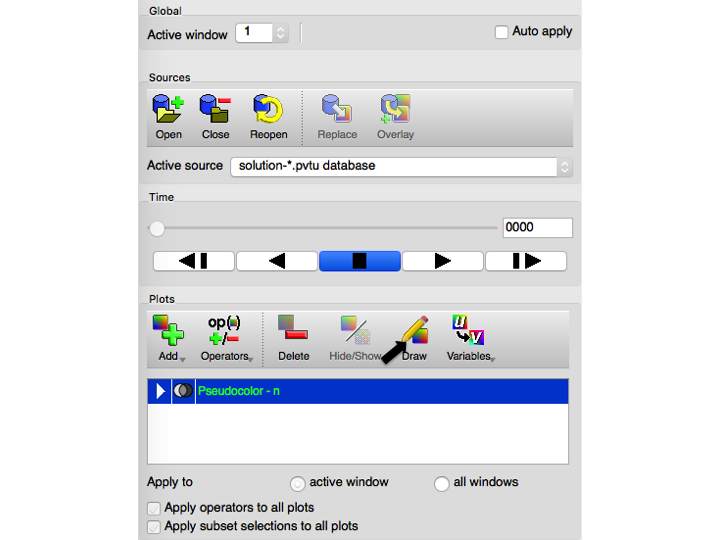
\includegraphics[width=0.7\textwidth]{visit_pseudocolor.png}
\vspace{0pt}
\end{figure}
The VisIt window will now have a plot of the initial condition of the order parameter:
\begin{figure}[H]
\vspace{0pt}
\centering
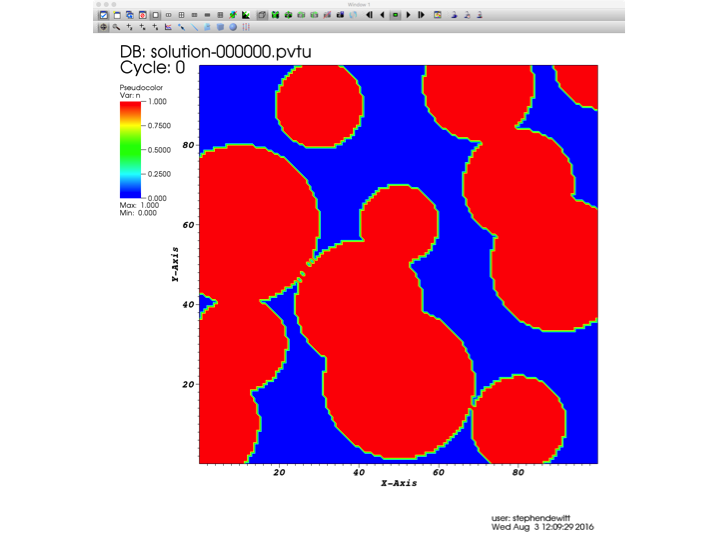
\includegraphics[width=0.7\textwidth]{visit_result.png}
\vspace{0pt}
\end{figure}
The result at other time steps can be visualized by dragging the time bar, or using the controls directly below the time bar. Dragging the time bar to the end will display the final result of the simulation:
\begin{figure}[H]
\vspace{0pt}
\centering
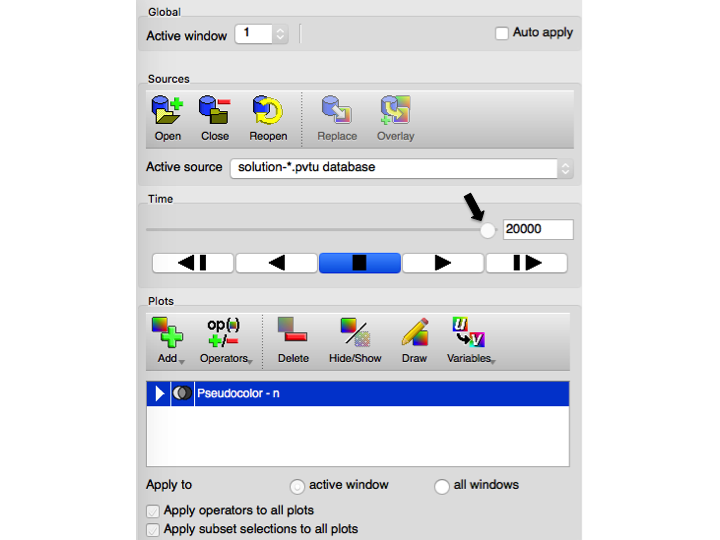
\includegraphics[width=0.7\textwidth]{visit_time_bar.png}
\vspace{0pt}
\end{figure}
\begin{figure}[H]
\vspace{0pt}
\centering
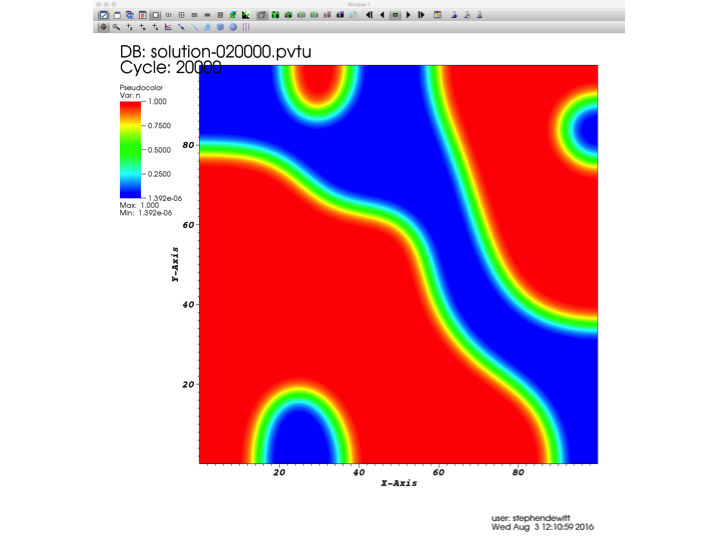
\includegraphics[width=0.7\textwidth]{visit_final_result.png}
\vspace{0pt}
\end{figure}

VisIt has a wide variety of capabilities for visualizing 1D, 2D, and 3D data, including postprocessing of output fields (e.g. to obtain derivatives of output fields or the result of mathematical expressions involving one or more output field). VisIt also has a powerful Python interface to provide scripting capabilities. More more instructions on how to use these, and other, features of VisIt, please consult the VisIt manual.

\subsection{Running the Other Example Applications}
Running the other example applications is as simple as going to the directory for the application of interest and repeating the steps in Section \ref{allen_cahn_instructions}. For example, to run the Cahn-Hilliard example application, when you are currently in the directory for the Allen-Cahn example application, you would type the following commands:
\begin{lstlisting}
$ cd ../cahnHilliard/ 
$ cmake . 
$ make debug 
$ mpirun -n 1 main 
\end{lstlisting}

\subsection{Running in Release Mode and with Multple Processors} \label{release_multicore}
Once you are sure that your code works as expected, you can compile it in ``Release Mode'', which is approximately 10x faster than ``Debug Mode''. However, no exceptions are checked in Release Mode and therefore the code may compile and run even if it contains several errors. Therefore, we strongly recommend that all new code is tested in Debug Mode before switching to Release Mode. To compile in Release mode, replace ``\$ make debug'' with ``\$ make release''.

One of the strengths of PRISMS-PF is that it can be run in parallel with almost no extra effort from the user. To run a simulation in parallel, replace the ``1'' in the ``mpirun'' command with the desired number of processor cores. The deal.II packages on their website already contain the MPI library, so no extra software has to be downloaded to use multiple cores.

From the directory of an example application, a simulation can be run in Release Mode on 4 cores using the following commands:
\begin{lstlisting}
$ cmake . 
$ make release
$ mpirun -n 4 main 
\end{lstlisting}

\section{Structure of a PRISMS-PF Application}
\subsection{Files in the Application Directories}
Each of the example application directories should contain at least eight files:
\begin{itemize}
\item parameters.in
\item equations.h
\item ICs\_and\_BCs.h
\item postprocess.h
\item customPDE.h
\item main.cc
\item formulation.pdf
\item CMakeLists.txt
\end{itemize}

It may contain two other files:
\begin{itemize}
\item postprocess.h
\item nucleation.h
\end{itemize}

The following section (Sec. \ref{parameters}) will discuss the structure and options for the input file, parameters.h. Users who do not need to change the governing equations or make other fundamental changes to the application will only need to modify this file.

Section \ref{app_files} discusses the structure of the files that define an application: equations.h, ICs\_and\_BCs.h, postprocess.h, nucleation.h, customPDE.h, and main.cc. Users who want to substantially modify existing PRISMS-PF applications or create their own will find this section useful.

The final two files in each application directory are formulation.pdf and CMakeLists.txt. The file formulation.pdf describes the mathematical formulation of the problem solved by the application. Finally, the file CMakeLists.txt is used by CMake to generate the makefile. Most users will not have any reason to change CMakeLists.txt.

\section{The Input File: parameters.in} \label{parameters}
Most PRISMS-PF users will spend the majority of their time interacting with the input file, parameters.h. This file allows users to specify the computational domain, the mesh, the time step parameters, the boundary conditions, the output, and model constants (and more). This file is read as a text file, so modifications to it do not require recompilation of the application.

Here is an example of an input file from the allenCahn application:
\scriptsize
\begin{lstlisting}
# Parameter list for the Allen-Cahn example application
# Refer to the PRISMS-PF manual for use of these parameters in the source code.

# =================================================================================
# Set the number of dimensions (2 or 3 for a 2D or 3D calculation)
# =================================================================================
set Number of dimensions = 2

# =================================================================================
# Set the length of the domain in all three dimensions
# (Domain size Z ignored in 2D)
# =================================================================================
# Each axes spans from zero to the specified length
set Domain size X = 100
set Domain size Y = 100
set Domain size Z = 100

# =================================================================================
# Set the element parameters
# =================================================================================
# The number of elements in each direction is 2^(refineFactor) * subdivisions
# Subdivisions Z ignored in 2D
# For optimal performance, use refineFactor primarily to determine the element size
set Subdivisions X = 1
set Subdivisions Y = 1
set Subdivisions Z = 1

set Refine factor = 8

# Set the polynomial degree of the element (allowed values: 1, 2, or 3)
set Element degree = 1

# =================================================================================
# Set the time step parameters
# =================================================================================
# The size of the time step
set Time step = 1.0e-2

# The simulation ends when either the number of time steps is reached or the
# simulation time is reached.
set Number of time steps = 5000

# =================================================================================
# Set the boundary conditions
# =================================================================================
# Set the boundary condition for each variable, where each variable is given by
# its name, as defined in equations.h. The four boundary condition
# types are NATURAL, DIRICHLET, NON_UNIFORM_DIRICHLET and PERIODIC. If all
# of the boundaries have the same boundary condition, only one boundary condition
# type needs to be given. If multiple boundary condition types are needed, give a
# comma-separated list of the types. The order is the miniumum of x, maximum of x,
# minimum of y, maximum of y, minimum of z, maximum of z (i.e left, right, bottom,
# top in 2D and left, right, bottom, top, front, back in 3D). The value of a
# Dirichlet BC is specfied in the following way -- DIRCHILET: val -- where 'val' is
# the desired value. If the boundary condition is NON_UNIFORM_DIRICHLET, the
# boundary condition should be specified in the appropriate function in 'ICs_and_BCs.h'.
# Example 1: All periodic BCs for variable 'c'
# set Boundary condition for variable c = PERIODIC
# Example 2: Zero-derivative BCs on the left and right, Dirichlet BCs with value
# 1.5 on the top and bottom for variable 'n' in 2D
# set Boundary condition for variable n = NATURAL, NATURAL, DIRICHLET: 1.5, DIRICHLET: 1.5

set Boundary condition for variable n = NATURAL

# =================================================================================
# Set the model constants
# =================================================================================
# Set the user-defined model constants, which must have a counter-part given in
# customPDE.h. These are most often used in the residual equations in equations.h,
# but may also be used for initial conditions and nucleation calculations. The type
# options currently are DOUBLE, INT, BOOL, TENSOR, and [symmetry] ELASTIC CONSTANTS
# where [symmetry] is ISOTROPIC, TRANSVERSE, ORTHOTROPIC, or ANISOTROPIC.

# The mobility, MnV in equations.h
set Model constant MnV = 1.0, DOUBLE

# The gradient energy coefficient, KnV in equations.h
set Model constant KnV = 2.0, DOUBLE

# =================================================================================
# Set the output parameters
# =================================================================================
# Type of spacing between outputs ("EQUAL_SPACING", "LOG_SPACING", "N_PER_DECADE",
# or "LIST")
set Output condition = EQUAL_SPACING

# Number of times the program outputs the fields (total number for "EQUAL_SPACING"
# and "LOG_SPACING", number per decade for "N_PER_DECADE", ignored for "LIST")
set Number of outputs = 5

# The number of time steps between updates being printed to the screen
set Skip print steps = 1000

\end{lstlisting}
\normalsize

The syntax for setting each input parameter is:
\begin{lstlisting}
set [parameter name] = [parameter value]
\end{lstlisting}
 The pound symbol (\#) is used for comments, and any text after it is ignored by the file parser.
 
 The following table lists all of the input parameters, seperated into the same groupings in the input file above:
 \footnotesize
 \renewcommand{\arraystretch}{1.5}
 \begin{center}
    \begin{tabular}{ | p{0.2\textwidth} | p{0.17\textwidth} | p{0.08\textwidth} | p{0.1\textwidth} | p{0.3\textwidth} |}
    \hline
      \multicolumn{5}{|c|}{\textbf{Dimensionality}} \\
    \hline
    \hline
    \emph{Name} & \emph{Options} & \emph{Required} & \emph{Default} & \emph{Description} \\ \hline
    Number of dimensions & 2, 3 & yes & n/a & The number of dimensions for the simulation.  \\ \hline
    \end{tabular}
\end{center}

\begin{center}
    \begin{tabular}{ | p{0.2\textwidth} | p{0.17\textwidth} | p{0.08\textwidth} | p{0.1\textwidth} | p{0.3\textwidth} |}
    \hline
      \multicolumn{5}{|c|}{\textbf{Compuational Domain}} \\
    \hline
    \hline
    \emph{Name} & \emph{Options} & \emph{Required} & \emph{Default} & \emph{Description} \\ \hline
    Domain size X & Any positive real number & yes & n/a & The size of the domain in the x direction. \\ \hline
     Domain size Y & Any positive real number & yes & n/a & The size of the domain in the y direction. \\ \hline
      Domain size Z & Any positive real number & yes & n/a & The size of the domain in the z direction. \\ \hline
    \end{tabular}
\end{center}

\begin{center}
    \begin{tabular}{ | p{0.2\textwidth} | p{0.17\textwidth} | p{0.08\textwidth} | p{0.1\textwidth} | p{0.3\textwidth} |}
    \hline
      \multicolumn{5}{|c|}{\textbf{Element Parameters}} \\
    \hline
    \hline
    \emph{Name} & \emph{Options} & \emph{Required} & \emph{Default} & \emph{Description} \\ \hline
    Subdivisions X & Any positive integer & no & 1 & The number of mesh subdivisions in the x direction to control the element aspect ratio. The mesh size is 2$^{(Refine Factor)}$ $\times$ Subdivisions in each direction.\\ \hline
     Subdivisions Y & Any positive integer & no & 1 & The number of mesh subdivisions in the y direction to control the element aspect ratio.The mesh size is 2$^{(Refine Factor)}$ $\times$ Subdivisions in each direction. \\ \hline
      Subdivisions Z & Any positive integer & no & 1 & The number of mesh subdivisions in the z direction to control the element aspect ratio. The mesh size is 2$^{(Refine Factor)}$ $\times$ Subdivisions in each direction.\\ \hline
      Refine factor & Any non-negative integer & yes & n/a & The number of initial refinements of the mesh. The mesh size is 2$^{(Refine Factor)}$ $\times$ Subdivisions in each direction. While in principle the mesh could be entirely controlled by the number of subdivisons, computational performance is best when the majority of the refinement is done via the Refine factor. \\ \hline
       Element degree & 1, 2, 3 & no & 1 & The polynomial order of the elements. The spatial order of accuracy is one plus the degree. \\ \hline
    \end{tabular}
\end{center}

\begin{center}
    \begin{tabular}{ | p{0.2\textwidth} | p{0.17\textwidth} | p{0.08\textwidth} | p{0.1\textwidth} | p{0.3\textwidth} |}
    \hline
      \multicolumn{5}{|c|}{\textbf{Mesh Adaptivity (Optional)}} \\
    \hline
    \hline
    \emph{Name} & \emph{Options} & \emph{Required} & \emph{Default} & \emph{Description} \\ \hline
    Mesh adaptivity & Boolean & no & false & Controls whether mesh adaptivity is enabled. \\ \hline
     Max refinement level & Any non-negative integer & no & -1 & The maximum number of local refinements during adaptive meshing. This parameter does not need to be specified if mesh adaptivity is disabled, but the default value will cause an error if mesh adaptivity is enabled. \\ \hline
      Min refinement level & Any non-negative integer & no & -1 & The minimum number of local refinements during adaptive meshing. This parameter does not need to be specified if mesh adaptivity is disabled, but the default value will cause an error if mesh adaptivity is enabled. \\ \hline
      Refinement criteria fields & Comma separated list of variable names & no & 0 & The indices of the variables that will determine the mesh refinement. The variable names are determined by the names given in equations.h.  \\ \hline
      Refinement window max & Comma separated list of real numbers & no &  & The mesh refines where the specified variables are between an upper and lower bound. This specifies the upper bound.  \\ \hline
        Refinement window min & Comma separated list of real numbers & no &  & The mesh refines where the specified variables are between an upper and lower bound. This specifies the lower bound.  \\ \hline
               Steps between remeshing operations & Positive integer & no & 1 & The number of time steps between mesh refinement operations. \\ \hline
    \end{tabular}
\end{center}

\begin{center}
    \begin{tabular}{ | p{0.2\textwidth} | p{0.17\textwidth} | p{0.08\textwidth} | p{0.1\textwidth} | p{0.3\textwidth} |}
    \hline
      \multicolumn{5}{|c|}{\textbf{Time Stepping}} \\
    \hline
    \hline
    \emph{Name} & \emph{Options} & \emph{Required} & \emph{Default} & \emph{Description} \\ \hline
    Time step & Any positive real number & yes & n/a & The time step size for the simulation. \\ \hline
Number of time steps & Any non-negative integer & no & -1 & The number of time steps until the simulation stops. Either this or the simulation end time must be specified. If both are specified, the simulation will end when the first condition is reached. \\ \hline
      Simulation end time & Any non-negative real number & no & -0.1 & The simulated time when until the simulation stops. Either this or the number of time steps must be specified. If both are specified, the simulation will end when the first condition is reached.  \\ \hline
    \end{tabular}
\end{center}

\begin{center}
    \begin{tabular}{ | p{0.2\textwidth} | p{0.17\textwidth} | p{0.08\textwidth} | p{0.1\textwidth} | p{0.3\textwidth} |}
    \hline
      \multicolumn{5}{|c|}{\textbf{Elliptic Solver Parameters (Optional)}} \\
    \hline
    \hline
    \emph{Name} & \emph{Options} & \emph{Required} & \emph{Default} & \emph{Description} \\ \hline
    Linear solver & SolverCG & no & SolverCG & Currently the only option is the deal.II conjugate gradient solver. \\ \hline
     Use absolute convergence tolerance & Boolean & no & false & Sets whether to use an absolute tolerance for the linear solver (versus a relative tolerance). \\ \hline
Solver tolerance value & Any positive real number & no & 1e-3 & The tolerance for the linear solver. If an absolute tolerance is used, the iterative solver stops when the L2 norm of the residual drops below the tolerance. If a relative tolerance is used, the iterative solver stops when the L2 norm of the residual has dropped by a factor equal to the tolerance. \\ \hline
Maximum allowed solver iterations & Any positive integer & no & 10000 & The maximum number of iterations for the linear solver, if this number of iterations is reached, the solver stops regardless of the tolerance value. \\ \hline
    \end{tabular}
\end{center}

\begin{center}
    \begin{tabular}{ | p{0.2\textwidth} | p{0.17\textwidth} | p{0.08\textwidth} | p{0.1\textwidth} | p{0.3\textwidth} |}
    \hline
      \multicolumn{5}{|c|}{\textbf{Output}} \\
    \hline
    \hline
    \emph{Name} & \emph{Options} & \emph{Required} & \emph{Default} & \emph{Description} \\ \hline
    Output condition & EQUAL\_SPACING, LOG\_SPACING, N\_PER\_DECADE, LIST & no & EQUAL \_SPACING & This sets the spacing between the times the simulation outputs the model variables. EQUAL\_SPACING spaces them equally, LOG\_SPACING spaces them  $10^{n/(outputs) \log(time steps)}$, N\_PER\_DECADE allows the user to set how many times the simulation outputs per power of ten iterations, and LIST outputs at a user-given list of time step numbers. \\ \hline
     Number of outputs & Any non-negative integer & no & 10 & The number of inputs if the output condition is EQUAL\_SPACING. The number of outputs if the output condition is N\_PER\_DECADE. Ignored for the other output conditions. \\ \hline
      List of time steps to output & Comma-separated list of non-negative integers & no & 0 & The list of time steps to output, used for the LIST output condition and ignored for the others. \\ \hline
Output file name (base) & String & no & solution & The name for the output file, before the time step and processor info are added. \\ \hline
Output file type & vtu, vtk & no & vtu & The output file type (currently limited to either vtu or vtk). \\ \hline
Skip print steps & Any positive integer & no & 1 & The number of time steps between updates to the terminal window (1 is every time step). \\ \hline
    \end{tabular}
\end{center}

\begin{center}
    \begin{tabular}{ | p{0.2\textwidth} | p{0.17\textwidth} | p{0.08\textwidth} | p{0.1\textwidth} | p{0.3\textwidth} |}
    \hline
      \multicolumn{5}{|c|}{\textbf{Boundary Conditions}} \\
    \hline
    \hline
    \emph{Name} & \emph{Options} & \emph{Required} & \emph{Default} & \emph{Description} \\ \hline
    Boundary condition for variable [variable name] & NATURAL, DIRICHLET, NON\_UNIFORM \_DIRICHLET, PERIODIC & yes & n/a & Sets the boundary condition for each scalar variable, using the variable name from equations.h. One line is required for each scalar  variable. See Note 1 below for details. \\ \hline
    Boundary condition for variable [variable name], component [direction] & NATURAL, DIRICHLET, NON\_UNIFORM \_DIRICHLET, PERIODIC & yes & n/a & Sets the boundary condition for each vector variable, using the variable name from equations.h. One line is required for each vector variable. See Note 1 below for details. \\ \hline
    \end{tabular}
\end{center}

\begin{center}
    \begin{tabular}{ | p{0.2\textwidth} | p{0.17\textwidth} | p{0.08\textwidth} | p{0.1\textwidth} | p{0.3\textwidth} |}
    \hline
      \multicolumn{5}{|c|}{\textbf{Loading Initial Conditions from File (Optional)}} \\
    \hline
    \hline
    \emph{Name} & \emph{Options} & \emph{Required} & \emph{Default} & \emph{Description} \\ \hline
    Load initial conditions & Comma-separated list of booleans & no & false & One true/false flag for each variable for whether the initial condition should be loaded from a vtk file. Currently, only scalar fields can be read in. SSee Note 2 below for details. \\ \hline
     Load parallel file & Comma-separated list of booleans & no & false & One true/false flag for each variable for whether each processor should read the initial conditions from a seperate file. See Note 2 below for details.  \\ \hline
      File names & Comma-separated list of strings & no &  & The name of the vtk file to be read for each variable, ignored for variables where the initial conditions isn't read in from a file. Often, all of the variables will read from the same vtk file. See Note 2 below for details.  \\ \hline
    \end{tabular}
\end{center}

\begin{center}
    \begin{tabular}{ | p{0.2\textwidth} | p{0.17\textwidth} | p{0.08\textwidth} | p{0.1\textwidth} | p{0.3\textwidth} |}
    \hline
      \multicolumn{5}{|c|}{\textbf{Nucleation (Optional}} \\
    \hline
    \hline
    \emph{Name} & \emph{Options} & \emph{Required} & \emph{Default} & \emph{Description} \\ \hline
    Nucleus semiaxes (x, y ,z) & Three positive real numbers & no &  & The semiaxes of the ellipsoidal nuclei to be seeded. See Note 3 below for details. \\ \hline
     Freeze zone semiaxes (x, y ,z) & Three positive real numbers & no &  & The semiaxes for the ellipsoidal region where the nucleus is frozen after seeding. See Note 3 below for details.  \\ \hline
      Freeze time following nucleation & Any non-negative real number & no & 0 & The amount of time the nucleus is frozen after seeding. See Note 3 below for details. \\ \hline
      Nucleation-free border thickness & Any non-negative real number & no & 0 & The size of the buffer region where nucleation is not allowed unless the boundary conditions are periodic. See Note 3 below for details. \\ \hline
      Minimum allowed distance between nuclei & Any non-negative real number & no & 2$\times$ the largest nucleus semiaxis  & The minimum allowed distance between nuclei centers during a single nucleation attempt. See Note 3 below for details. \\ \hline
      Minimum allowed distance between nuclei & Any non-negative real number & no & 2$\times$ the largest nucleus semiaxis  & The minimum allowed distance between nuclei centers during a single nucleation attempt. See Note 3 below for details. \\ \hline
      Order parameter cutoff value & Any non-negative real number & no & 0.01  & The minimum allowed value of the sum of all nucleating variable fields where nucleation is allowed to occur. Implemented to prevent nucleation inside existing particles. See Note 3 below for details. \\ \hline
      Time steps between nucleation attempts & Any positive integer & no & 100  & The number of time steps between nucleation attempts. See Note 3 below for details. \\ \hline
    \end{tabular}
\end{center}

\begin{center}
    \begin{tabular}{ | p{0.2\textwidth} | p{0.17\textwidth} | p{0.08\textwidth} | p{0.1\textwidth} | p{0.3\textwidth} |}
    \hline
      \multicolumn{5}{|c|}{\textbf{Model constants (Optional)}} \\
    \hline
    \hline
    \emph{Name} & \emph{Options} & \emph{Required} & \emph{Default} & \emph{Description} \\ \hline
    Model constant [constant name] & value followed by a comma then a type & no &  & Sets the value of a constant defined for that particular application. The allowed types are DOUBLE, INT, BOOL, TENSOR, and [symmetry] ELASTIC CONSTANTS where [symmetry] is ISOTROPIC, TRANSVERSE, ORTHOTROPIC, or ANISOTROPIC. See Note 4 below for details. \\ \hline
    \end{tabular}
\end{center}

\normalsize

\textbf{Note 1 (Boundary Conditions):} \\
The boundary condition must be set for each variable, where each variable is given by its name, as defined in equations.h. The four boundary condition types are NATURAL, DIRICHLET, NON\_UNIFORM\_DIRICHLET and PERIODIC. If all of the boundaries have the same boundary condition, only one boundary condition type needs to be given. If multiple boundary condition types are needed, give a comma-separated list of the types. The order is the miniumum of x, maximum of x, minimum of y, maximum of y, minimum of z, maximum of z (i.e left, right, bottom, top in 2D and left, right, bottom, top, front, back in 3D). The value of a Dirichlet BC is specfied in the following way -- DIRCHILET: val -- where 'val' is the desired value. If the boundary condition is NON\_UNIFORM\_DIRICHLET, the boundary condition should be specified in the appropriate function in 'ICs\_and\_BCs.h'. For vector variables, one boundary condition should be specified for each component.

Example 1: All periodic BCs for variable 'c'
\begin{lstlisting}
set Boundary condition for variable c = PERIODIC
\end{lstlisting}

Example 2: Zero-derivative BCs on the left and right, Dirichlet BCs with value 1.5 on the top and bottom for variable 'n' in 2D
\begin{lstlisting}
set Boundary condition for variable n = NATURAL, NATURAL, DIRICHLET: 1.5,
 DIRICHLET: 1.5
\end{lstlisting}

Example 3: All periodic BCs for the y component of the vector variable 'u'
\begin{lstlisting}
set Boundary condition for variable u, component y = PERIODIC
\end{lstlisting}

\textbf{Note 2 (Loading Initial Conditions from File):} \\
Currently, initial conditions can only be read from vtk files (\emph{not} vtu files). Some variables can have initial conditions read from file and others can be specified in ICs\_and\_BCs.h in the same application. For each variable, the user must set whether the file(s) to be read are in serial format, where all processors read from the same file, or parallel format, where all processors read from different files. If parallel format is selected, the desired domain decomposition must between the files and the simulation to be run. For non-adaptive meshes this will be true if the same number of cores is the same between the simulation that generated the vtk files and the simulation reading the vtk files. For adaptive meshes, obtaining the same domain decomposition may be difficult and merging parallel vtk files into a single file is likely the best approach. This process is planned to be cleaner in future versions of PRISMS-PF. An example of loading inital conditions from file can be seen in the `allenCahn\_pfield' application.

\textbf{Note 3 (Nucleation):} \\
PRISMS-PF includes the capability for explicitly placing nuclei over the course of a simulation using an approach similar to the one described in the following publication: \\
Jokisaari, Permann, and Thornton, A nucleation algorithm for the coupled conserved-nonconserved phase field model, \emph{Computational Materials Science}, 112, (2016). \\
A nucleus of an non-conserved order parameter is placed within the computational domain determined by a probability given by the `getNucleationProbability' function in the `nucleation.h' file. The variables that are allowed to nucleate are specified in the `loadVariableAttributes' function in the `equations.h' file, as are the variable values needed to calculate the nucleation probability. The determination of when and where a nucleus should be seeded is determined in the core PRISMS-PF library, but the actual placement of the nucleus by modifying one of the model fields is expected to be performed in the `residualRHS' function in the `equations.h' file. The mobility for the nucleated field should be set to zero in the region surrounding the nucleus (the ``freeze zone'') for a specified amount of time (the ``freeze time''). Examples of nucleating particles can be found in the nucleationModel and preferential\_nucleationModel applications.

\textbf{Note 4 (Model constants):} \\
Each application specifies its own set of model constants. These are most often used in the residual equations in the `equations.h' file, although they may also be used to specify initial conditions, non-uniform Dirichlet boundary conditions, nucleation probabilties, etc. Currently, five types of model constants are accepted: DOUBLE, INT, BOOL, TENSOR, and ELASTIC CONSTANTS. The use of these different types is as follows:
\begin{itemize}
\item DOUBLE: For individual real numbers
\item INT: For individual integers
\item BOOL: For individual booleans (true/false)
\item TENSOR: For either rank 1 tensors (i.e. vectors) or rank 2 tensors (i.e. matrices) with a size of the number of dimensions. These are assumed to be real numbers. Each row should be given by a comma-separated list in parentheses. For example, a 3D vector would be given as ``(2.5, 1.2, 0.1)'' and a 2D matrix would be given as: ``((4.1, 2.0),(1.6, 5.2))''.
\item {[symmetry]} ELASTIC CONSTANTS: For sets of elastic constants, given as a vector. The symmetry options are ISOTROPIC, TRANSVERSE, ORTHOTROPIC, or ANISOTROPIC. The number of entries for the different symmetries are given below. PRISMS-PF converts these sets of elastic constants into a stiffness matrix.
\end{itemize}

The number and order of the entries for the elastic constants are (where C$_{ij}$ are entries in the stiffness matrix):
\begin{itemize}
\item ISOTROPIC (2D/3D): 2 constants (Young's Modulus, Poisson's Ratio)
\item TRANSVERSE (3D): 5 constants (C$_{11}$, C$_{33}$, C$_{44}$, C$_{12}$, C$_{13}$)
\item ORTHOTROPIC (3D): 9 constants (C$_{11}$, C$_{22}$, C$_{33}$, C$_{44}$, C$_{55}$, C$_{66}$, C$_{12}$, C$_{13}$, C$_{23}$)
\item ANISOTROPIC (2D/3D): 21 constants (C$_{11}$, C$_{22}$, C$_{33}$, C$_{44}$, C$_{55}$, C$_{66}$, C$_{12}$, C$_{13}$, C$_{14}$, C$_{15}$, C$_{16}$, C$_{23}$, C$_{24}$, C$_{25}$, C$_{26}$, C$_{34}$, C$_{35}$, C$_{36}$, C$_{45}$, C$_{46}$, C$_{56}$)
\end{itemize}

Each model constant in `parameters.in' must have a counterpart in the appropriate section of the `customPDE.h' file. 



\section{The Application Files: equations.h, ICs\_and\_BCs.h, postprocess.h, nucleation.h, customPDE.h, and main.cc} \label{app_files}
This section details the files that define each application. The norm is that substantial modifications to these files consistute a new application (in contrast to simply making changes to `parameters.in'. Modifying these files may require some knowledge of C++.

A very brief description of the purpose of each of these files is below, an in-depth discussion can be found in the following subsections:
\begin{itemize}
\item equations.h: Specifies the attributes of the model variables and the model's residual equations
\item ICs\_and\_BCs.h: Specifies the initial conditions for each variable (unless the initial condition is read from file) and non-uniform Dirichlet boundary conditions, if applicable.
\item postprocess.h: Specifies variable other than the primary model variables to output, as well as the expressions to derive these variables.
\item nucleation.h: Contains the function that determines the probability density of nucleation.
\item customPDE.h: Contains the prototypes of the functions for the application, also contains declarations of the model constants given in `parameters.h'.
\item main.cc: Main C++ function that controls the flow of the simulation. Identical for all the example applications and it is unlikely that users will need to modify it.
\end{itemize}

\subsection{equations.h} \label{equations}
The file ``equations.h'' contains a list of the variables in the model equations and their attributes as well as the residuals for the model equations. The file contains three functions: \emph{loadVariableAttributes}, \emph{residualRHS}, and \emph{residualLHS}. 

To modify the functions in this file, one needs to be familar with the weak form of the governing equations (hereafter referred to as the residual equations). In PRISMS-PF, the residual equations are expressed in two terms. The first is the part of the integrand that is multiplied by the test function. The second is the part of the integrand that multipled by the gradient of the test function. For the coupled Cahn-Hilliard/Allen-Cahn system, the residual equations are 
\begin{align}
  \int_{\Omega}   w  \eta^{n+1}  ~dV &=\int_{\Omega}  w  \left( \underbrace{\eta^{n} - \Delta t M_{\eta}~ ((f_{\beta,c}^n-f_{\alpha,c}^n)H_{,\eta}^n)}_{r_{\eta}} \right)+ \nabla w \cdot \underbrace{(- \Delta t M_{\eta}\kappa) \nabla \eta^{n}}_{r_{\eta x}} ~dV 
\end{align}
and 
\begin{align}
  \int_{\Omega}   w  c^{n+1}  ~dV = &\int_{\Omega}   w \underbrace{c^{n}}_{r_c} \\&+  \nabla w   \underbrace{(-\Delta t M_{c})~ [~(f_{\alpha,cc}^n(1-H^{n+1})+f_{\beta,cc}^n H^{n+1}) \nabla c + ~((f_{\beta,c}^n-f_{\alpha,c}^n)H^{n+1}_{,\eta} \nabla \eta) ] }_{r_{cx}} ~dV
\end{align}
for the Allen-Cahn and Cahn-Hilliard equation, respectively. Each of the residual terms is marked with an underbrace. The terms multiplied by the test function are referred to as the value residual terms and the terms multiplied by the gradient of the test function are referred to as the gradient residual terms.

\subsubsection{loadVariableAttributes}
Here is the \emph{loadVariableAttributes} function for the coupled Allen-Cahn/Cahn-Hilliard example application:
\scriptsize
\begin{lstlisting}
// =================================================================================
// Set the attributes of the primary field variables
// =================================================================================
void variableAttributeLoader::loadVariableAttributes(){
	// Variable 0
	set_variable_name		(0,''c'');
	set_variable_type		(0,SCALAR);
	set_variable_equation_type	(0,PARABOLIC);

	set_need_value			(0,true);
	set_need_gradient		(0,true);
	set_need_hessian		(0,false);

	set_need_value_residual_term	(0,true);
	set_need_gradient_residual_term	(0,true);

  	// Variable 1
	set_variable_name		(1,''n'');
	set_variable_type		(1,SCALAR);
	set_variable_equation_type	(1,PARABOLIC);

	set_need_value			(1,true);
	set_need_gradient		(1,true);
	set_need_hessian		(1,false);

	set_need_value_residual_term	(1,true);
	set_need_gradient_residual_term	(1,true);
}
\end{lstlisting}
\normalsize

This function specifies the model variables and their attributes. In this case, the two model variables are the concentration, ``c'', and the order parameter, ``n''. Here, ``c'' is listed as the zeroth variable and ``n'' is listed as the first. For each variable, a series of attributes are set using a series of C++ function calls. The following table lists the functions and a description of the attributes they set:

\footnotesize
\begin{center}
    \begin{tabular}{ | p{0.25\textwidth} | p{0.13\textwidth}| p{0.08\textwidth} | p{0.11\textwidth} | p{0.29\textwidth} |}
    \hline
    \emph{Function}  & \emph{Options} & \emph{Required} & \emph{Default} & \emph{Description} \\ \hline
    set\_variable\_name & String & no & var  & Sets the name of the variable. This name is used in `parameters.in' as well as during output. \\ \hline
    set\_variable\_type & SCALAR, VECTOR & no & SCALAR  & Sets whether the variable is a scalar or a vector. \\ \hline
    set\_variable\_equation\_type & PARABOLIC, ELLIPTIC & no & PARABOLIC  & Sets whether the govenring equation for the variable is a parabolic or ellpitic PDE. \\ \hline
    set\_need\_value & Boolean & no & true  & Sets whether the value of the variable is needed in the function \emph{residualRHS} below. \\ \hline
    set\_need\_gradient & Boolean & no & true & Sets whether the gradient of the variable is needed in the function \emph{residualRHS} below. \\ \hline
    set\_need\_hessian & Boolean & no & false & Sets whether the hessian of the variable is needed in the function \emph{residualRHS} below. \\ \hline
    set\_need\_need\_value \_residual\_term & Boolean & no & false & Sets whether the residual equation has a value residual term. \\ \hline
    set\_need\_need\_gradient \_residual\_term & Boolean & no & false & Sets whether the residual equation has a gradient residual term. \\ \hline
    set\_need\_value\_LHS & Boolean & no & false  & Sets whether the value of the variable is needed in the function \emph{residualLHS} below. (Only needed for elliptic PDEs). \\ \hline
    set\_need\_gradient\_LHS & Boolean & no & false & Sets whether the gradient of the variable is needed in the function \emph{residualLHS} below. (Only needed for elliptic PDEs). \\ \hline
    set\_need\_hessian\_LHS & Boolean & no & false & Sets whether the hessian of the variable is needed in the function \emph{residualLHS} below. (Only needed for elliptic PDEs). \\ \hline
    set\_need\_need\_value \_residual\_term\_LHS & Boolean & no & false & Sets whether the LHS residual equation has a value residual term. (Only needed for elliptic PDEs). \\ \hline
    set\_need\_need\_gradient \_residual\_term\_LHS & Boolean & no & false & Sets whether the LHS residual equation has a gradient residual term. (Only needed for elliptic PDEs). \\ \hline
    set\_allowed\_to\_nucleate & Boolean & no & false & Sets whether the nucleation algorithms should be activated for this variable. (Only needed when nucleation is desired). \\ \hline
    set\_need\_value\_nucleation & Boolean & no & false & Sets whether the value of the variable is needed to calculate the nucleation probability in the `nucleation.h' file. (Only needed when nucleation is desired). \\ \hline
    \end{tabular}
\end{center}
\normalsize

\footnotesize
\begin{center}
    \begin{tabular}{ | p{0.25\textwidth} | p{0.13\textwidth}| p{0.08\textwidth} | p{0.11\textwidth} | p{0.29\textwidth} |}
    \hline
    \emph{Function}  & \emph{Options} & \emph{Required} & \emph{Default} & \emph{Description} \\ \hline
    set\_need\_value\_pp & Boolean & no & true  & Sets whether the value of the variable is needed in the function \emph{postProcessedFields} in `postprocess.h'. \\ \hline
    set\_need\_gradient\_pp & Boolean & no & true & Sets whether the gradient of the variable is needed in the function \emph{postProcessedFields} in `postprocess.h'. \\ \hline
    set\_need\_hessian\_pp & Boolean & no & true & Sets whether the hessian of the variable is needed in the function \emph{postProcessedFields} in `postprocess.h'. \\ \hline
    \end{tabular}
\end{center}
\normalsize

Some of these function calls are not present in the `equations.h' file for the coupledCahnHilliardAllenCahn application. Use of the LHS function calls can be found in the preciptiateEvolution application (among others) and use the nucleation function calls can be found the nucleationModel and preferential\_nucleationModel applications.

\subsubsection{residualRHS}
Here is the \emph{residualRHS} function for the coupled Allen-Cahn/Cahn-Hilliard example application:
\scriptsize
\begin{lstlisting}
// =================================================================================
// residualRHS
// =================================================================================
// This function calculates the residual equations for each variable. It takes
// "variable_list" as an input, which is a list of the value and derivatives of
// each of the variables at a specific quadrature point. The (x,y,z) location of
// that quadrature point is given by "q_point_loc". The function outputs residuals
// to variable_list. The index for each variable in this list corresponds to
// the index given at the top of this file.
template <int dim, int degree>
void customPDE<dim,degree>::residualRHS(
		variableContainer<dim,degree,dealii::VectorizedArray<double> > & variable_list,
		 dealii::Point<dim, dealii::VectorizedArray<double> > q_point_loc) const {

//c
scalarvalueType c = variable_list.get_scalar_value(0);
scalargradType cx = variable_list.get_scalar_gradient(0);

//n
scalarvalueType n = variable_list.get_scalar_value(1);
scalargradType nx = variable_list.get_scalar_gradient(1);

// Free energy for each phase and their first and second derivatives
scalarvalueType faV = (-1.6704-4.776*c+5.1622*c*c-2.7375*c*c*c+1.3687*c*c*c*c);
scalarvalueType facV = (-4.776 + 10.3244*c - 8.2125*c*c + 5.4748*c*c*c);
scalarvalueType faccV = (10.3244-16.425*c+16.4244*c*c);
scalarvalueType fbV = (5.0*c*c-5.9746*c-1.5924);
scalarvalueType fbcV = (10.0*c-5.9746);
scalarvalueType fbccV = constV(10.0);

// Interpolation function and its derivative
scalarvalueType hV = (10.0*n*n*n-15.0*n*n*n*n+6.0*n*n*n*n*n);
scalarvalueType hnV = (30.0*n*n-60.0*n*n*n+30.0*n*n*n*n);

// Residual equations
scalargradType muxV = ( cx*((1.0-hV)*faccV+hV*fbccV) + nx*((fbcV-facV)*hnV) );
scalarvalueType rcV = c;
scalargradType rcxV = (constV(-McV*userInputs.dtValue)*muxV);
scalarvalueType rnV = (n-constV(userInputs.dtValue*MnV)*(fbV-faV)*hnV);
scalargradType rnxV = (constV(-userInputs.dtValue*KnV*MnV)*nx);

// Residuals for the equation to evolve the concentration 
variable_list.set_scalar_value_residual_term(0,rcV);
variable_list.set_scalar_gradient_residual_term(0,rcxV);

// Residuals for the equation to evolve the order parameter
variable_list.set_scalar_value_residual_term(1,rnV);
variable_list.set_scalar_gradient_residual_term(1,rnxV);

}
\end{lstlisting}
\normalsize

In this function the residuals at a particular quadrature point are calculated. The inputs to this function are a list of the model variable values and derivatives, \emph{variable\_list} and a point giving access to (x,y,z) coordinates, \emph{q\_point\_loc}. The residual terms are added to \emph{variable\_list} as the output. The first few lines of the function set more convienent names for the variables and their derivatives. By convention, the value of the variable is denoted by the variable name (\emph{c} for the concentration and \emph{n} for the structural order parameter in this case), the list of first derivatives is denoted by the variable name followed by an ``x'', and second derivatives are denoted by the variable name followed by ``xx''. Each variable in \emph{variable} can be accessed by the index it was given in \emph{loadVariableAttributes}. The variable value and the derivatives can be accessed through the \emph{get\_scalar\_value},  \emph{get\_scalar\_gradient}, and \emph{get\_scalar\_hessian} object members for scalar variables and the  \emph{get\_vector\_value},  \emph{get\_vector\_gradient}, and \emph{get\_vector\_hessian} functions. The data type for the value of a scalar variable is \emph{scalarvalueType} (a scalar), the data type for the first derivatives of a scalar variable is \emph{scalargradType} (a vector with a length equal to the number of dimensions), and the data type for the second derivatives of a scalar variable is \emph{scalarhessType} (a matrix with a size equal to the number of dimensions by the number of dimensions). For vector variables, the data types are \emph{vectorvalueType} (a vector with length equal to the number of dimensions), \emph{vectorgradType} (a matrix with a size equal to the number of dimensions by the number of dimensions), and \emph{vectorgradType} (a rank-three tensor with a size in each direction equal to the number of dimensions).

After the nicknames for the field variables are set, the residual terms are calculated (including some intermediate variables, such as the free energies and the interpolation functions in the example above). These use the same six data types discussed in the preceding paragraph. The model variables given in `parameters.h' can be used to define the residual terms.

Finally, the residuals for the governing equations are submitted to \emph{variable\_list}, using the functions \emph{set\_scalar\_value\_residual\_term}, \emph{set\_scalar\_gradient\_residual\_term}, \emph{set\_vector\_value\_residual\_term}, and \emph{set\_vector\_gradient\_residual\_term}, once again referring the variables by their index.

The nickname step can be skipped, if desired, although the code is generally more readable with nicknames (and the performance overhead is minimal). An example without nicknames for the fields can be found in the grainGrowth application, where loops over the ten variables are easier to construct when not declaring all of the variables at once. One word of caution, though: calling \emph{set\_scalar\_value\_residual\_term} and \emph{set\_scalar\_gradient\_residual\_term} overwrites the value and gradient of the variable, respectively (and same for the variants for vectors). Thus, either the residuals need to be cached and then set after all the residuals have been calculated (as is done in the grainGrowth application) or the values and gradients need to be cached before setting the residuals (as is done with the standard nicknaming approach). 

\fbox{
\parbox{\textwidth}{
\textbf{A Note on Types:} The deal.II library uses a data structure called a VectorizedArray to store the variable values and their derivatives. This data structured in optimized for modern vectorized processors, giving a substantial speedup in some cases. However, this data structure can complicate things slightly. One complicating factor is that VectorizedArrays can't always be added, subtracted, multiplied, or divided with more standard data types like doubles. For this reason, you will see the ``constV(arguement)'' function scattered throughout the code. This function turns a non-VectorizedArray into a VectorizedArray. To be safe, you can always encase non-VectorizedArrays with ``constV()'' when they share an operation with a VectorizedArray. A second complication is that not all of the standard mathematical operations are available for VectorizedArrays. The basic trigonometric functions are available, as are exponentials and square roots. However, hyperbolic tangents are not. If needed, they must be constructed from exponents. A third complication is that conditional statements involving VectorizedArrays are not allowed. VectorizedArrays contain data from multiple points that the processor operates on at once. Under normal conditions a conditional statement could only be applied to one of the points in the VectorizedArray. There are possible ways to break up the VectorizedArrays and work on the pieces of data individually, but this approach is not recommended for most users. Clever use of ``max'' and ``min'' functions (which do exist for VectorizedArrays) may be able to take the place of a conditional statement. For more details on the deal.II implementation of VectorizedArrays (including a list of mathematical operations that are allowed), please visit: \\
https://www.dealii.org/8.4.0/doxygen/deal.II/classVectorizedArray.html}}

\subsubsection{residualLHS}
In the coupledCahnHilliardAllenCahn, the \emph{residualLHS} function is empty because it is only needed for elliptic PDEs (or more specifically, when a non-trivial matrix inversion needs to be performed). Here is the \emph{residualLHS} function from the precipitateEvolution application, where the equation for mechanical equilibrium is elliptic.

From the formulation file in the precipitateEvolution application, the residual equation for the mechanical displacement is:
\begin{gather}
R =  \int_{\Omega}   \nabla w :  C(\eta_1, \eta_2, \eta_3) : \left( \epsilon - \epsilon^0(c,\eta_1, \eta_2, \eta_3)\right) ~dV = 0 
\end{gather}

To turn this equation into a matrix inversion problem, we can linearize it with Newton's method. (It can also be directly written as a matrix inversion problem. For historical purposes we do the linearization and for some mundane reasons, non-zero Dirichlet boundary conditions do not currently work with that approach. Therefore, for the meantime, we recommend the approach below.) The solution $u$ is found through the following expression, given an initial guess $u_0$: 
\begin{gather}
0 = R(u) = R(u_0 + \Delta u)
\end{gather}
where $\Delta u = u - u_0$. Then, applying the discretization that $u = \sum_i N^i U^i$, where $N^i$ is the i$^{th}$ shape function, we can write the following linearization:
\begin{equation}
\frac{\delta R(u)}{\delta u} \Delta U = -R(u_0) \label{matrix_eqn}
\end{equation}
The discretized form of this equation can be written as a matrix inversion problem. However, in PRISMS-PF, we only care about the product $\frac{\delta R(u)}{\delta u} \Delta U$. Taking the variational derivative of $R(u)$ yields:
\begin{align}
\frac{\delta R(u)}{\delta u} &= \frac{d}{d\alpha} \int_{\Omega}   \nabla w :C: \left[ \epsilon (u+\alpha w) - \epsilon^0 \right] ~dV  \bigg{|}_{\alpha=0} \\
&=  \int_{\Omega}   \nabla w :C: \frac{1}{2}\frac{d}{d\alpha}\left[ \nabla(u+\alpha w) + \nabla(u+\alpha w)^T  - \epsilon^0\right] ~dV \bigg{|}_{\alpha=0}\\
&= \int_{\Omega}   \nabla w :C: \frac{d}{d\alpha} \left[ \nabla(u+\alpha w) - \epsilon^0 \right]  ~dV \bigg{|}_{\alpha=0} \quad (due ~to ~the ~symmetry ~of ~C) \\
&= \int_{\Omega}   \nabla w :C: \nabla w  ~dV 
\end{align}
In its discretized form $\frac{\delta R(u)}{\delta u} \Delta U$ is:
\begin{equation}
\frac{\delta R(u)}{\delta u} \Delta U = \sum_i \sum_j \int_{\Omega} \nabla N^i : C : \nabla N^j dV ~\Delta U^j
\end{equation}
Moving back to the non-discretized form yields:
\begin{equation}
\frac{\delta R(u)}{\delta u} \Delta U = \int_{\Omega} \nabla w : C : \nabla (\Delta u) dV
\end{equation}
Thus, the full equation relating $u_0$ and $\Delta u$ is:
\begin{equation}
\int_{\Omega} \nabla w : \underbrace{C : \nabla (\Delta u)}_{r_{ux}^{LHS}} dV = -\int_{\Omega}   \nabla w : \underbrace{(\epsilon-\epsilon^0)}_{r_{ux}} ~dV
\end{equation}
The above values of $r_{ux}^{LHS}$ and $r_{ux}$ are used to define the residuals in the equations.h file. A similar process can be undertaken for other elliptic problems.

The \emph{residualLHS} function from the preciptiateEvolution application is:
\scriptsize
\begin{lstlisting}
// =================================================================================
// residualLHS (needed only if at least one equation is elliptic)
// =================================================================================
// This function calculates the residual equations for the iterative solver for
// elliptic equations.for each variable. It takes "modelVariablesList" as an input,
// which is a list of the value and derivatives of each of the variables at a
// specific quadrature point. The (x,y,z) location of that quadrature point is given
// by "q_point_loc". The function outputs "modelRes", the value and gradient terms of
// for the left-hand-side of the residual equation for the iterative solver. The
// index for each variable in these lists corresponds to the order it is defined at
// the top of this file (starting at 0), not counting variables that have
// "need_val_LHS", "need_grad_LHS", and "need_hess_LHS" all set to "false". If there
// are multiple elliptic equations, conditional statements should be used to ensure
// that the correct residual is being submitted. The index of the field being solved
// can be accessed by "this->currentFieldIndex".
template <int dim, int degree>
void customPDE<dim,degree>::residualLHS(
	variableContainer<dim,degree,dealii::VectorizedArray<double> > & variable_list,
	dealii::Point<dim, dealii::VectorizedArray<double> > q_point_loc) const {

//n1
scalarvalueType n1 = variable_list.get_scalar_value(1);

//n2
scalarvalueType n2 = variable_list.get_scalar_value(2);

//n3
scalarvalueType n3 = variable_list.get_scalar_value(3);

//u
vectorgradType ux = variable_list.get_vector_gradient(4);
vectorgradType ruxV;

// Interpolation functions

scalarvalueType h1V = (10.0*n1*n1*n1-15.0*n1*n1*n1*n1+6.0*n1*n1*n1*n1*n1);
scalarvalueType h2V = (10.0*n2*n2*n2-15.0*n2*n2*n2*n2+6.0*n2*n2*n2*n2*n2);
scalarvalueType h3V = (10.0*n3*n3*n3-15.0*n3*n3*n3*n3+6.0*n3*n3*n3*n3*n3);

// Take advantage of E being simply 0.5*(ux + transpose(ux)) and use the dealii "symmetrize" function
dealii::Tensor<2, dim, dealii::VectorizedArray<double> > E;
E = symmetrize(ux);

// Compute stress tensor (which is equal to the residual, Rux)
if (n_dependent_stiffness == true){
	dealii::Tensor<2, CIJ_tensor_size, dealii::VectorizedArray<double> > CIJ_combined;
	CIJ_combined = CIJ_Mg*(constV(1.0)-h1V-h2V-h3V) + CIJ_Beta*(h1V+h2V+h3V);

	computeStress<dim>(CIJ_combined, E, ruxV);
}
else{
	computeStress<dim>(CIJ_Mg, E, ruxV);
}

variable_list.set_vector_gradient_residual_term(4,ruxV);

}

\end{lstlisting}
\normalsize

Like \emph{residualRHS}, \emph{residualLHS} takes \emph{variables\_list} and  \emph{q\_point\_loc} as inputs. However, because only one elliptic equation is solved at a time, the output are the residual terms for a single residual. As in \emph{residualRHS}, the model variable values and derivatives are given convienent names at the start of the file. Similar to \emph{residualRHS}, the value of \emph{ruxV} is set and then used to set the appropriate residual for \emph{variables\_list} (in this case the vector residual term for the fourth variable).

If multiple elliptic equations need to be solved, you will need to use conditional statements to calculate the proper residual depending on the elliptic equation being solved. The index of the field being solved can be accessed using the ``this-$>$currentFieldIndex'' statement. 

\subsection{IC\_and\_BCs.h}
The `ICs\_and\_BCs.h' file contains four functions: \emph{InitialCondition}, \emph{InitialConditionVec}, \emph{NonUniformDirichletBC}, and \emph{NonUniformDirichletBCVec}. The first two functions in the file are used to set the initial conditions for scalar and vector variables, respectively, while the third and fourth functions set non-uniform Dirichlet boundary conditions for scalar and vector variables, respectively. For all of these functions, most users should only need to modify the sections between the lines.  

\subsubsection{InitialCondition and InitialConditionVec}
Here's a look at the \emph{InitialCondition} function for the coupled Allen-Cahn/Cahn-Hilliard example application:
\scriptsize
\begin{lstlisting}
template <int dim>
double InitialCondition<dim>::value (const Point<dim> &p, const unsigned int component) const
{
	  double scalar_IC = 0;
	  // --------------------------------------------------------------------------
	  // ENTER THE INITIAL CONDITIONS HERE FOR SCALAR FIELDS
	  // --------------------------------------------------------------------------
	  // Enter the function describing conditions for the fields at point "p".
	  // Use "if" statements to set the initial condition for each variable
	  // according to its variable index.

	  // The initial condition is two circles/spheres defined
	  // by a hyperbolic tangent function. The center of each circle/sphere is
	  // given by "center" and its radius is given by "rad".

	  double center[2][3] = {{1.0/3.0,1.0/3.0,1.0/3.0},{3.0/4.0,3.0/4.0,3.0/4.0}};
	  double rad[12] = {userInputs.domain_size[0]/5.0, userInputs.domain_size[0]/12.0};
	  double dist;
	  scalar_IC = 0;

	  if (index == 0){
		  scalar_IC = 0.009;
	  }

	  for (unsigned int i=0; i<2; i++){
		  dist = 0.0;
		  for (unsigned int dir = 0; dir < dim; dir++){
			  dist += (p[dir]-center[i][dir]*userInputs.domain_size[dir])
			  		*(p[dir]-center[i][dir]*userInputs.domain_size[dir]);
		  }
		  dist = std::sqrt(dist);

		  // Initial condition for the concentration field
		  if (index == 0){
			  scalar_IC += 0.5*(0.125)*(1.0-std::tanh((dist-rad[i])/(1.0)));
		  }
		  else {
			  scalar_IC += 0.5*(1.0-std::tanh((dist-rad[i])/(1.0)));
		  }
	  }

	  // --------------------------------------------------------------------------
	  return scalar_IC;
}
\end{lstlisting}
\normalsize

In this function, the variable \emph{scalarIC} should be set to the desired intitial condition. The (x,y,z) coordinates can be accessed by the \emph{p} variable, with indices zero through 2. For example, if you wanted to initialize a field to $5xy$, you would enter:
\tiny
\begin{lstlisting} 
scalarIC = 5.0 * p[0] * p[1];
\end{lstlisting} \normalsize
The initial conditions given above are a bit more complicated. They set the initial conditions for two circular (spherical in 3D) particles. The initial condition for different variables is set using conditional statements and the \emph{index} variable. The \emph{index} variable refers to the variable index from the top of the ``equations.h''. This example uses conditional statements to set the initial conditions differently for the concentration (\emph{index}==0) and the structural order parameter  (\emph{index}==0). The initial conditions for both fields are calculated using hyperbolic tangent functions that make use of the distance between the centers of the particles and the point \emph{p}.

The model constants defined in `parameters.in' can be used in the intial condition or boundary condition functions. However, the syntax is the same as in `customPDE.h', not as in the residual functions. That is, they have to be extracted from the \emph{userInputs} object. An example of this is in the dendriticSolidification application, where \emph{deltaV} is set using one of the model constants.

Similarly, the initial conditions for vector fields are set in \emph{InitialConditionsVec}. Here is the (somewhat trivial) \emph{InitialConditionVec} function for the precipitateEvolution example application:
\scriptsize
\begin{lstlisting}
template <int dim>
void InitialConditionVec<dim>::vector_value (
	const dealii::Point<dim> &p,
	dealii::Vector<double> &vector_IC) const
{
	  // --------------------------------------------------------------------------
	  // ENTER THE INITIAL CONDITIONS HERE FOR VECTOR FIELDS
	  // --------------------------------------------------------------------------
	  // Enter the function describing conditions for the fields at point "p".
	  // Use "if" statements to set the initial condition for each variable
	  // according to its variable index.

	  if (index==4){
		  vector_IC(0) = 0.0;
		  vector_IC(1) = 0.0;
          if (dim == 3){
        	  vector_IC(2) = 0.0;
          }
	  }
	  // --------------------------------------------------------------------------
}
\end{lstlisting}
\normalsize
The initial condition for each component is set using the \emph{vector\_IC} variable, where parentheses are used to select the x, y, or z component.

\subsubsection{NonUniformDirichletBC and NonUniformDirichletBCVec}
These functions are needed when one or more boundaries are set to NON\_UNIFORM\_DIRICHLET. These functions are very similar to the initial condition functions above, the user sets an expression for \emph{scalar\_BC} or \emph{vector\_BC} at point \emph{p}. Once again, the variable \emph{index} is used to differentiate between variables based on their index from the top of the `equations.h' file. For Dirichlet boundary conditions that vary in time, the current time can be accessed via the variable \emph{time}.

Currently, the one of the only two applications that use a non-uniform Dirichlet boundary condition is CHiMaD\_benchmark6a (the other is CHiMaD\_benchmark6b). Here is the \emph{NonUniformDirichletBC} function from CHiMaD\_benchmark6a:
\scriptsize
\begin{lstlisting}
template <int dim>
double NonUniformDirichletBC<dim>::value (
	const dealii::Point<dim> &p, 
	const unsigned int component) const
{
    double scalar_BC=0;
    // --------------------------------------------------------------------------
    // ENTER THE NON-UNIFORM DIRICHLET BOUNDARY CONDITIONS HERE FOR SCALAR FIELDS
    // --------------------------------------------------------------------------
    // Enter the function describing conditions for the fields at point "p".
    // Use "if" statements to set the boundary condition for each variable
    // according to its variable index. This function can be left blank if there
    // are no non-uniform Dirichlet boundary conditions.
    
    if (index == 2){
        if (direction == 1){
            double x=p[0];
            double y=p[1];
            scalar_BC=std::sin(y/7.0);
        }
    }
    // -------------------------------------------------------------------------
    return scalar_BC;
}
\end{lstlisting}
\normalsize

\subsection{postprocess.h}
Unlike the files discussed so far in this section, the `postprocess.h' file is optional. This file allows users to specify fields other than the primary model variable to output. It also includes an option to integrate over a field variable (e.g. to check conservation of a field). In the example problems, this file is often used to calculate the total free energy of the system, which should be monotonically decreasing for most phase field problems. It also is convienent for calculating somewhat complicated expressions such as chemical potentials, stresses, and strains.

Note: Two restrictions are currently in place for the postprocessor. First, postprocessing variables can only be scalars, not vectors. Second, the postprocessor won't work if the primary model variable with index zero is a vector. (This is because postprocessor uses the mesh of the zeroth primary variable to calculate and output the postprocessed field.) These restrictions will be lifted in future versions of PRISMS-PF.

\subsubsection{loadPostProcessorVariableAttributes}
Similar to the `equations.h' file, `postprocess.h' begins with a function called \emph{loadPostProcessorVariableAttributes}, which sets the attributes of the postprocessing variables. Here is the \emph{loadPostProcessorVariableAttributes} function from the coupledCahnHilliardAllenCahn application, where the postprocessed field is ``f\_tot'', the total free energy:
\scriptsize
\begin{lstlisting}
void variableAttributeLoader::loadPostProcessorVariableAttributes(){

	// Variable 0
	set_variable_name		(0,"f_tot");
	set_variable_type		(0,SCALAR);

	set_need_value_residual_term	(0,true);
	set_need_gradient_residual_term	(0,false);

    	set_output_integral         	(0,true);

}
\end{lstlisting}
\normalsize

As in `equations.h', a series of attributes for each variable are set using a series of C++ function calls. The following table lists the functions and a description of the attributes they set:
\footnotesize
\begin{center}
    \begin{tabular}{ | p{0.25\textwidth} | p{0.13\textwidth}| p{0.08\textwidth} | p{0.11\textwidth} | p{0.29\textwidth} |}
    \hline
    \emph{Function}  & \emph{Options} & \emph{Required} & \emph{Default} & \emph{Description} \\ \hline
    set\_variable\_name & String & no & var  & Sets the name of the variable. \\ \hline
    set\_variable\_type & SCALAR, VECTOR & no & SCALAR  & Sets whether the variable is a scalar or a vector (Currently only scalar fields are allowed). \\ \hline
    set\_need\_need\_value \_residual\_term & Boolean & no & false & Sets whether the expression for the postprocessed field has a value residual term. \\ \hline
    set\_need\_need\_gradient \_residual\_term & Boolean & no & false & Sets whether the expression for the postprocessed field has a gradient residual term. \\ \hline
    set\_output\_integral & Boolean & no & false & Sets whether the integrated value of the postprocessed field is calculated. The integrated value is output to the file `integratedFields.txt'. \\ \hline
    \end{tabular}
\end{center}
\normalsize

\subsubsection{postProcessedFields}
The second function in the `postprocess.h' file is similar to the residual functions in `equations.h'. The primary difference is that, while the primary model fields are read in from \emph{variable\_list}, the residuals are submitted to \emph{pp\_variable\_list}. Otherwise, the structure is similar and expressions can be copied from one function to another.

Here is the \emph{postProcessedFields} from the coupledCahnHilliardAllenCahn application:
\scriptsize
\begin{lstlisting}
template <int dim,int degree>
void customPDE<dim,degree>::postProcessedFields(const variableContainer<dim,degree,dealii::VectorizedArray<double> > & variable_list,
				variableContainer<dim,degree,dealii::VectorizedArray<double> > & pp_variable_list,
												const dealii::Point<dim, dealii::VectorizedArray<double> > q_point_loc) const {

//c
scalarvalueType c = variable_list.get_scalar_value(0);

//n
scalarvalueType n = variable_list.get_scalar_value(1);
scalargradType nx = variable_list.get_scalar_gradient(1);

// Free energy for each phase
scalarvalueType faV = (-1.6704-4.776*c+5.1622*c*c-2.7375*c*c*c+1.3687*c*c*c*c);
scalarvalueType fbV = (5.0*c*c-5.9746*c-1.5924);

// Interpolation function
scalarvalueType hV = (10.0*n*n*n-15.0*n*n*n*n+6.0*n*n*n*n*n);

// The homogenous free energy
scalarvalueType f_chem = (constV(1.0)-hV)*faV + hV*fbV;

// The gradient free energy
scalarvalueType f_grad = constV(0.5*KnV)*nx*nx;

// The total free energy
scalarvalueType f_tot;
f_tot = f_chem + f_grad;

// Residuals for the equation to evolve the order parameter 
pp_variable_list.set_scalar_value_residual_term(0, f_tot);


}
\end{lstlisting}
\normalsize

\subsection{nucleation.h}
The `nucleation.h' file is also an optional file that is only needed when explcit nucleation is needed for the application. It contains the function \emph{getNucleationProbability}, which calculates the probability of nucleation in a given volume element \emph{dV} at a particular point in space \emph{p} at time \emph{this-$>$currentTime}. Please refer to Note 3 in Sec. \ref{parameters} for a description of the nucleation model in PRISMS-PF.

The values of the primary field variables can be accessed through the \emph{variable\_value} input, using the variable index from `equations.h'. Only variables where \emph{set\_need\_value\_nucleation} was set to true the \emph{loadVariableAttributes} function in `equations.h' can be accessed.

Here is \emph{getNucleationProbability} from the nucleationModel application:
\scriptsize
\begin{lstlisting}
template <int dim, int degree>
double customPDE<dim,degree>::getNucleationProbability(variableValueContainer variable_value, double dV, dealii::Point<dim> p) const
{
//Supersaturation factor
double ssf;
if (dim ==2) ssf=variable_value(0)-calmin;
if (dim ==3) ssf=(variable_value(0)-calmin)*(variable_value(0)-calmin);
	
// Calculate the nucleation rate
double J=k1*exp(-k2/(std::max(ssf,1.0e-6)))*exp(-tau/(this->currentTime));
double retProb=1.0-exp(-J*userInputs.dtValue*((double)userInputs.steps_between_nucleation_attempts)*dV);
   	
return retProb;
}
\end{lstlisting}
\normalsize

\subsection{customPDE.h}
The final header file in each application folder is `customPDE.h'. This file contains the declarations for all of the functions and variables specific to the application. In C++ terminology, it is the declaration for the customPDE class, which is a subclass of MatrixFreePDE. For most users, the relevant section is labeled as ``Model constants specific to this subclass'', which is where the model constants from `parameters.in' are extracted from the \emph{userInputs} object. There is a separate function to extract constants of each type. These are:
\begin{itemize}
\item get\_model\_constant\_double
\item get\_model\_constant\_int
\item get\_model\_constant\_bool
\item get\_model\_constant\_rank\_1\_tensor
\item get\_model\_constant\_rank\_2\_tensor
\item get\_model\_constant\_elasticity\_tensor
\end{itemize}

Each of these take the variable name from `parameters.in' as an input and output the appropriate type.

Here is `customPDE.h' from the preciptiateEvolution application, where all of the different types of constants are used:
\scriptsize
\begin{lstlisting}
#include "../../include/matrixFreePDE.h"

template <int dim, int degree>
class customPDE: public MatrixFreePDE<dim,degree>
{
public:
	customPDE(userInputParameters<dim> _userInputs): 
		MatrixFreePDE<dim,degree>(_userInputs) , userInputs(_userInputs) {};

private:
	#include "../../include/typeDefs.h"

	const userInputParameters<dim> userInputs;

	// Pure virtual method in MatrixFreePDE
	void residualRHS(
		variableContainer<dim,degree,dealii::VectorizedArray<double> > & variable_list,
		dealii::Point<dim, dealii::VectorizedArray<double> > q_point_loc) const;

	// Pure virtual method in MatrixFreePDE
	void residualLHS(
		variableContainer<dim,degree,dealii::VectorizedArray<double> > & variable_list,
		dealii::Point<dim, dealii::VectorizedArray<double> > q_point_loc) const;

	// Virtual method in MatrixFreePDE that we override if we need postprocessing
	#ifdef POSTPROCESS_FILE_EXISTS
	void postProcessedFields(
		const variableContainer<dim,degree,dealii::VectorizedArray<double> > & variable_list,
		variableContainer<dim,degree,dealii::VectorizedArray<double> > & pp_variable_list,
		const dealii::Point<dim, dealii::VectorizedArray<double> > q_point_loc) const;
	#endif

	// Virtual method in MatrixFreePDE that we override if we need nucleation
	#ifdef NUCLEATION_FILE_EXISTS
	double getNucleationProbability(variableValueContainer variable_value, double dV) const;
	#endif

	// ================================================================
	// Methods specific to this subclass
	// ================================================================


	// ================================================================
	// Model constants specific to this subclass
	// ================================================================

	double McV = userInputs.get_model_constant_double("McV");
	double Mn1V = userInputs.get_model_constant_double("Mn1V");
	double Mn2V = userInputs.get_model_constant_double("Mn2V");
	double Mn3V = userInputs.get_model_constant_double("Mn3V");
	dealii::Tensor<2,dim> Kn1 = userInputs.get_model_constant_rank_2_tensor("Kn1");
	dealii::Tensor<2,dim> Kn2 = userInputs.get_model_constant_rank_2_tensor("Kn2");
	dealii::Tensor<2,dim> Kn3 = userInputs.get_model_constant_rank_2_tensor("Kn3");
	bool n_dependent_stiffness = userInputs.get_model_constant_bool("n_dependent_stiffness");
	dealii::Tensor<2,dim> sfts_linear1 = userInputs.get_model_constant_rank_2_tensor("sfts_linear1");
	dealii::Tensor<2,dim> sfts_const1 = userInputs.get_model_constant_rank_2_tensor("sfts_const1");
	dealii::Tensor<2,dim> sfts_linear2 = userInputs.get_model_constant_rank_2_tensor("sfts_linear2");
	dealii::Tensor<2,dim> sfts_const2 = userInputs.get_model_constant_rank_2_tensor("sfts_const2");
	dealii::Tensor<2,dim> sfts_linear3 = userInputs.get_model_constant_rank_2_tensor("sfts_linear3");
	dealii::Tensor<2,dim> sfts_const3 = userInputs.get_model_constant_rank_2_tensor("sfts_const3");
	double A4 = userInputs.get_model_constant_double("A4");
	double A3 = userInputs.get_model_constant_double("A3");
	double A2 = userInputs.get_model_constant_double("A2");
	double A1 = userInputs.get_model_constant_double("A1");
	double A0 = userInputs.get_model_constant_double("A0");
	double B2 = userInputs.get_model_constant_double("B2");
	double B1 = userInputs.get_model_constant_double("B1");
	double B0 = userInputs.get_model_constant_double("B0");

	const static unsigned int CIJ_tensor_size =2*dim-1+dim/3;
	dealii::Tensor<2,CIJ_tensor_size> CIJ_Mg = 
		userInputs.get_model_constant_elasticity_tensor("CIJ_Mg");
	dealii::Tensor<2,CIJ_tensor_size> CIJ_Beta = 
		userInputs.get_model_constant_elasticity_tensor("CIJ_Beta");



	// ================================================================

};

\end{lstlisting}
\normalsize

This file can also be used to declare new member functions for the application. One example of this is the \emph{seedNucleus} function in the nucleationModel application.

Furthermore, for advanced users, the customPDE class can be used to override MatrixFreePDE functions from the core PRISMS-PF library. One example of this is in the CHiMaD\_benchmark6b application, where the \emph{makeTriangulation} function is overridden to create a non-square mesh.

\subsection{main.cc}
The final file in the application directory is the C++ `main.cc' file. This file controls the overall flow of the code and is unlikely to be modified by most users. For all of the example applications, `main.cc' is identical. One situation where a user may want to modify `main.cc' is if they wanted to run several simulations with different parameter sets for one execution of the code.

\section{Tests}
The `tests' folder in the root directory contains some tests to ensure that PRISMS-PF is working properly. A battery of automated tests can be found in the `automated\_tests' directory. These can be run by running the python script `run\_automatic\_tests.py'. This will run a series of unit and regression tests, printing a summary of the results to the screen and writing to the file `test\_results.txt'. This python file can also be used as an example of automating PRISMS-PF simulations.

The `unit\_tests' directory contains a driver for a series of unit tests. To run them enter:
\begin{lstlisting}
$ cmake . 
$ make debug 
$ mpirun -n 1 main 
\end{lstlisting}
A summary of the tests will print to the screen.

\section{Creating Custom Applications}
You can create your own PRISMS-PF applications by making simple modifications to the input files described in the previous section. To create a new application, simply create a new folder in the applications directory and copy the files from a related example application. \textbf{If the file ``CMakeCache.txt'' exists, delete it} (this file contains paths to the original application, and if left would cause the compiler to compile the code from the original application). Then, make your desired modifications (changing the initial or boundary conditions, changing the residual equations, etc.) and compile and run your application the same way you would one of the example applications.

Once your have your own applications running, we'd love to help you share them with the community. Please contact us at prismsphasefield.dev@umich.edu if you need help using GitHub to generate a pull request so that we can add your work to the public repository.

\end{document}
